\documentclass{article}

\usepackage[paperheight=11in,paperwidth=8.5in,top=1.5in,bottom=1.5in,right=1in,left=1in]{geometry}

\usepackage{url}
\usepackage[latin1]{inputenc}
\usepackage[dvips]{graphicx}

%%%%%%%%%%%%%%%%%%%%%%%%%%%%%%%%%%%%%%%%%%%%%%%%%%%%%%%%%%%%%%%%%%%%%%%%%%%%%%
% front page
%%%%%%%%%%%%%%%%%%%%%%%%%%%%%%%%%%%%%%%%%%%%%%%%%%%%%%%%%%%%%%%%%%%%%%%%%%%%%%

\begin{document}

%\begin{frontmatter}


\title{Parallelizing Evolutionary Algorithms on GPUs:\\ Methodology and Trends}

%% use optional labels to link authors explicitly to addresses:
%% \author[label1,label2]{}
%% \address[label1]{}
%% \address[label2]{}

\author{Gustavo Romero$^1$, M.G. Arenas$^1$, P.A. Castillo$^1$,\\ 
A.M. Mora$^1$, P. Garc�a-S�nchez$^2$, J.J. Merelo$^1$\\ \\
\small{$^1$ Dept. Computer Architecture and Computer Technology,}\\
\small{ETSIIT-CITIC, University of Granada (Spain)}\\
\small{$^2$ Dept. Computer Engineering, University of C�diz (Spain)}\\
\small{\texttt{\{gustavo,mgarenas,pacv,amorag,jmerelo\}@ugr.es}}\\ \small{\texttt{pablo.garciasanchez@uca.es}}
} 

\maketitle

%%%%%%%%%%%%%%%%%%%%%%%%%%%%%%%%%%%%%%%%%%%%%%%%%%%%%%%%%%%%%%%%%%%%%%%%%%%%%%
% abstract
%%%%%%%%%%%%%%%%%%%%%%%%%%%%%%%%%%%%%%%%%%%%%%%%%%%%%%%%%%%%%%%%%%%%%%%%%%%%%%

\begin{abstract}
Metaheuristics and bioinspired methods have been widely adapted to General Purpose Graphics Processing Units (GPGPUs). Among them, Evolutionary Algorithms (EAs) stand out since they are inherently parallel structures based on a population of independent agents. Due to this reason there are many different distributed schemes for EAs.
This paper describes the parallelization methodologies usually applied to EAs, and presents a survey on the literature related to their application on GPGPUs.
The paper also includes a review of advances in hardware and software along with new trends in the field.
Thus, more than 200 associated publications, from the last 13 years, have been revised and their properties have been extracted: type of EA implemented, hybridization, configuration and whether they have been applied to solve real world problems. 
We also define a taxonomy of the approaches used for parallelization on the literature. Then, a more in-depth analysis has been conducted on a wide selection, also describing the most representative in each category. 
As a remark, Genetic Algorithms, the most widely used EAs, have been frequently applied to real world problems due to the advantages that GPGPUs offer.
% Antonio - TODO: complete with more conclusions...
\end{abstract}

%\begin{keyword}
%parallel computation \sep evolutionary algorithms \sep metaheuristics \sep GPUs \sep GPGPUs \sep survey
%\end{keyword}
%
%\end{frontmatter}

%% main text

%%%%%%%%%%%%%%%%%%%%%%%%%%%%%%%%%%%%%%%%%%%%%%%%%%%%%%%%%%%%%%%%%%%%%%%%%%%%%%
\section{Introduction}
\label{sec:intro}
%%%%%%%%%%%%%%%%%%%%%%%%%%%%%%%%%%%%%%%%%%%%%%%%%%%%%%%%%%%%%%%%%%%%%%%%%%%%%%

The application of Evolutionary Algorithms to obtain the solution of
many real world problems or large instances of some benchmark problems
requires a high amount of computational power. In order to deal with
them, parallelization of this kind of algorithms has been performed
with the main objective of reducing the computational time whereas,
eventually, the quality of the solutions is improved. 

%******** Antonio - TO DO: Revise and rewrite/integrate this with the other text
Initially the EAs were proposed as a sequential set of steps with different operators and data structures. Then, several ways to parallelize these algorithms were presented, with new schemes and operations. Nowadays, new emerging trends that deal with new technologies (such as P2P or Cloud Computing) and new algorithmic methods (such as parameter adaptation) are being used. 
These trends require a new way to develop EAs taking into account some shortcomings, such as integration of heterogeneous elements or dynamic resources, and also to deal with fault-tolerance, churn, massive
scalability or decentralization.
%********

These algorithms
were usually executed in one or more central processing units (CPUs)
each one with one or more cores. However the advances in the video
game industry have led to the production of low cost and
high-performance graphics processing units (GPUs) included in almost
every PC nowadays and also in most of the mobile devices.  % There are
                                % weird words here. Are you trying to
                                % change the text by using synonyms?
                                % - Jj

GPUs are specialized stream processors, initially designed for rendering graphics in all kind of applications, but specially games. Typically, a GPU is able to perform graphics manipulations at a much higher speed than a general purpose CPU, since the graphics processor is specifically designed to handle certain primitive operations which occur frequently in graphics applications. Internally, the GPU contains a number of small processors that are used to perform calculations.

Depending on the power of a GPU, the number of threads that can be executed in parallel on such devices is currently in the order of hundreds to thousands and this number is expected to be increased every year. Nowadays, developers can write their own high-level programs on GPU. Due to the wide availability, programmability, and high-performance of these consumer-level GPUs, they are cost-effective for, not just game playing, but also scientific computing.

Since some years ago, GPUs are exposed to the programmer as a set of general-purpose shared-memory Single Instruction Multiple Data (SIMD) multi-core processors. This makes these architectures well suited to run large or complex computational problems in parallel.
Thus, nowadays, these units are used as general-purpose processors, and leveraged as powerful substitutes or complements for CPUs in many problem solving frameworks.

General-purpose computing on graphics processing units (GPGPU) consists in the use of a Graphics Processing Unit (GPU), which typically handles computer graphics related calculus, to perform any kind of computation traditionally carried out by a central processing unit (CPU). Recently there has been a growing interest in GPU computation, due to the fact that this kind of processors has the ability to perform massive and restricted parallel processing, which is very attractive to researchers with applications that require intensive parallel computation.

EAs \cite{EAs_Back96} are a class of probabilistic search and optimisation algorithms inspired on the model of Darwinistic evolution. 
There are several subtypes, depending on the data structure that is preferentially used for representing solutions, but Genetic Algorithms (GAs) \cite{GAs_Goldberg89} and Genetic Programming (GP) \cite{GP_Koza92} are the most extended. The main features are common to all of them: a population of individuals or potential solutions of the target problem, a selection method that favours better solutions, and a set of operators that act upon the
selected solutions. Thus, after an initial population is created, usually randomly, the selection and operators - crossover and mutation - are applied to the individuals, and the new population then replaces the older one. This is repeated for a number of generations or until another stop condition is met. 
If there is defined a correct {\em fitness function}, which assigns a reliable value to every individual, this process guarantees that the average quality of the population increases with the number of generations.

EAs present a structure which is inherently parallel because the individuals of the population are relatively independent. They work independently, but all of them cooperate to find a solution. Thus, their distribution on different computation nodes is quite straight and not very difficult to implement. Normally every node is devoted to work on a subpopulation or island \cite{Cantu-Paz_parallel_GAs}. In the finest-grained models, or fully distributed, every node is assigned to one individual \cite{Tomassini_fully_distributed_EAs}.

The aim of the parallelization is usually the improvement of the running time for yielding an objective solution, if known, or for obtaining a certain degree of quality in the solution, if it is not the optimal. Sometimes this distribution could also imply a different searching scheme, which can lead to a different searching area of the space of solutions and thus, to a different solution or set of solutions for an optimization problem, which, in turn, could be better than the one obtained in a sequential approach.
For these reasons, EAs are so far the most prolific metaheuristic in terms of existing parallel approaches, including the recent distribution on GPUs, by means of the new parallelization paradigm which we focus on here.

Thus, the paper presents a survey of the most extended evolutionary algorithms and the different proposals of GPUs-parallelization approaches made in a number of research works. They are organized according to a parallelization taxonomy, which is also introduced.
In addition, this work describes the features and advantages of GPGPUs, then it explains the general approaches to use and profit a GPGPU model, and gives an overview of currently available programming tools and software systems.

The rest of the paper is structured as follows: Next section presents GPUs as highly parallel devices architectures. Then, a background on the different
higher level programming languages used to take advantage on GPUs is described. The following section proposes a taxonomy based on the different parallel structures implemented in the literature, in order to categorize all the papers.
Then, a set of representative works describing different approaches using GPUs are reviewed and divided following the proposed taxonomy. Finally, some conclusions are remarked in the last section.


%%%%%%%%%%%%%%%%%%%%%%%%%%%%%%%%%%%%%%%%%%%%%%%%%%%%%%%%%%%%%%%%%%%%%%%%%%%%%%%
\section{Evolutionary Algorithms}
\label{sec:eas}
%%%%%%%%%%%%%%%%%%%%%%%%%%%%%%%%%%%%%%%%%%%%%%%%%%%%%%%%%%%%%%%%%%%%%%%%%%%%%%%

This section gives a general overview of the most used types of Evolutionary Algorithms (EAs) describing their common elements. In addition, the most extended models to parallelize EAs are presented, to understand all their possible architectural possibilities. 

% ------------------------------------------------------------------------------
\subsection{Description}
\label{subsec:eas-description}

Evolutionary Algorithms are a set of bioinspired techniques applied to optimization problems \cite{eiben2010whatis}, based on the process of natural selection \cite{darwin1859}. In this kind of pseudo-stochastic algorithms, a \textit{population} of codified solutions (called \textit{individuals}) is created. There is also a \textit{fitness} function, which evaluates the level of adaptation of the individuals to the problem to solve.
Thus, the fittest individuals have more chances to be selected for reproduction, so their offspring could inherit their genetic material. 


%\subsection{Types of Evolutionary Algorithms}
%\label{sec:distributed:types}
The general scheme of an EA, extracted from the work by Eiben and Smith \cite{eiben2010whatis} is described in Figure \ref{fig:basicscheme}.  

\begin{figure}[tb]
\begin{verbatim}
BEGIN
 INITIALISE population with random candidate solutions;
 EVALUATE each candidate;
 REPEAT UNTIL (TERMINATION CONDITION is satisfied) DO
   1 SELECT parents;
   2 RECOMBINE pairs of parents;
   3 MUTATE the resulting offspring;
   4 EVALUATE new candidates;
   3 SELECT individuals for the next generation;
 OD
END
\end{verbatim}
\caption{General scheme of an evolutionary algorithm in pseudo-code}
\label{fig:basicscheme}
\end{figure}

Although most of the EAs follow this structure, there are some differences depending on the representation of solutions, the operators to apply, or even the kind of problem to solve. Thus, according to the book \cite{eiben2003introduction}, the classical types  of EAs are:

%A possible classification is presented in this section, taking into account the new approaches that cannot fit with the traditional taxonomy. This classification would help to clarify the elements that  distinguish an algorithm from another (for example, the operators), and the existing similarities and differences, in order to establish a good starting point to classify EAs in GPGPUs.

%\subsection{Classic classification of EAs}
%\label{subsec:classicEAs}
%EAs are usually classified using a traditional variant, according to
%the book of Eiben and Smith \cite{eiben2003introduction}. These authors clarify that the features of an EA are:
%\begin{itemize}
%\item EAs are population-based.
%\item EAs mostly uses recombination to generate new individuals from the existing ones.
%\item EAs are stochastic.
%\end{itemize}


\begin{description}
\item [Genetic Algorithms] These kind of algorithms were proposed by Holland \cite{holland1975adaptation}, and later `refined' by Goldberg \cite{goldberg1988genetic}. In this kind of EA, the representation of the solution is a string of numbers (normally binary), called \textit{chromosome}. The individuals are selected proportionally to their fitness, and then \textit{recombination} and/or \textit{mutation} are applied to generate new individuals that will be included in the population (replacing some other). %These algorithms have been used in different areas, such as function optimization \cite{michalewicz1996genetic}, combinatorial optimization \cite{Esparcia2009EVITA}, artificial intelligence in videogames \cite{Fernandez20111optimizing}, or generative art \cite{Garcia2013RGB}, among others. 

\item[Evolution Strategies] The Evolution Strategies (ES) are applied to solve problems whose solution is included in the domain of real numbers. Their main difference with GAs is the consideration of a self-adaptation of the mutation rate, being coded in each individual \cite{eiben2005shared}. In addition, the parent selection is conducted randomly, instead of being based on the fitness. %ES have been applied in fields such as Evolutionary Robotics \cite{Garcia2012testing}.

% Antonio - TO DO: fix this description. ;)
\item[Evolutionary Programming] In Evolutionary Programming (EP), the representation of every solution is usually another algorithm, so it depends on the nature of the problem being solved, for example, neural networks \cite{Castillo1999gprop} or Radial Basis Functions (RBFs) \cite{Gonzalez2003multiobjective} have been used as individuals.

\item[Genetic Programming] The objective of this technique is to
  generate (and evolve) functions or programs to solve specific
  problems. Each individual is represented in the form of a tree,
  composed by operators (or {\em primitives}) and variables ({\em
    terminals}). These sets are usually fixed and known in advance. 
  The genome size is, therefore, variable, but there is frequently a maximum size for the individuals, in order to avoid too high evaluation costs. %GP has been used to evolve LISP (LISt Processing) programs   \cite{Koza1990Tools}, or XSLT (eXtensible Stylesheet     Language Transformations) scripts \cite{Garcia2008XSLT}, among  others.

\end{description}

%\subsection{Other models}

However, there are other EAs that do not match in the previous classification. For example \textit{Differential Evolution} (DE) \cite{storn1997differential}, \textit{Estimation of Distribution Algorithms} (EDAs) \cite{larranaga2002estimation} or \textit{Bayesian Optimization Algorithms} (BOAs) \cite{pelikan2005bayesian}. 

Differential Evolution \cite{storn1997differential} also exploits a population of potential solutions. Three individuals are selected randomly from the population to create \textit{random noisy vectors}. These vectors are recombined with the initial random individuals to create the \textit{trial vectors}. They are compared one by one with the original vectors and the best of each comparison is kept for the next generation.

% Antonio - TO DO: describe EDAs and BOAs... or not describe EDAs... or swap EDAs by EP in the list above. :D

Table \ref{tab:summaryEAs} shows the main differences between all these types of EAs. Note that we have selected the common features of each algorithm. For example, the replacement in GAs can be different from the generational one, or the representation can also be a real-value vector. 

\begin{table}
\resizebox{17cm}{!}{
\begin{tabular}{|p{3cm}|p{3cm}|p{3cm}|p{3cm}|p{3cm}|p{3cm}|}
\hline
				& GA 	 & ES  & EP & GP & DE  \\
\hline\hline
Representation  & Usually finite alphabet strings & Real-value vectors  & Problem-depending					& Tree 				& Real-value vectors 	 \\
Initialization  & \multicolumn{5}{c}{Random, depending of the problem and individual structure} 						 \\
Selection 	& Fitness proportional 	& Random 				& 						& Fitness proportional & Random to create noisy vectors \\
Recombination   & Genome crossover		& Genome crossover		& 						& Sub-tree exchange		& Random gene by gene			\\
Mutation  		& Random 				& Gaussian perturbation	& 						& Random 				& Implicit in the noisy vectors	 \\
Replacement		& Generational			& ($\mu,\lambda$) or ($\mu + \lambda$) &			& Generational 			& Compared with the original	 \\
\hline
\end{tabular}
}
\caption{Differences between the types of EAs \cite{eiben2003introduction}.}
\label{tab:summaryEAs}
\end{table}


% Antonio - TO DO: add a brief description of other parellelization models, such as P2P or Cloud Computing-based ones. We could add our own cites (Juanlu's and Maribel's/JJ's).


% ------------------------------------------------------------------------------
\subsection{Models of Parallel and Distributed Evolutionary Algorithms}
\label{subsec:eas-distributed:parallel}

Evolutionary Algorithms are inherently parallelizable, since each individual can be considered as an independent unit \cite{Alba13parallel}. Thus, in principle, there are several possible ways to parallelize them: for example, fitness evaluation can be conducted in several slave machines, or the population can be distributed among different nodes to be evolved at the same time. 

Two main types of parallelization models for EAs were classified by Alba and Tomassini in \cite{Alba02Parallelism}: \textit{Global parallel EAs} and
\textit{Spatially structured EAs}. However, with the arise of new
technologies and architectures, such as P2P or Cloud Computing, new ways of parallelization of EAs were proposed. 


%\subsubsection{Traditional parallelization classification}

This classification is still the most extended, even if it was established in 2002, however, it does not consider issues such as fault-tolerance, churn, massive scalability or decentralization. So, the number of computational nodes are considered constant during the whole execution and both the network and the nodes are reliable and trustworthy. Since a GPGPU is a kind of stable and reliable architecture, we consider the classification also as valid for the purposes of this paper.

% ----------------------------------------
\subsubsection{Global parallel evolutionary algorithms} 
In this model, also called \textit{Farming model}, \textit{Master-Slave} or \textit{Centralized EA}, the parallelism is applied at evaluation level. Thus, a central node coordinates several slave nodes. This node executes the EA in a sequential way, but it distributes the individuals of the population among the slaves just for being evaluated. Figure \ref{fig:masterslave} depicts this approach.

\begin{figure}[tb]
\centering
%\includegraphics[width=20pc]{gfx/distributed/masterslave.jpg}
\includegraphics[width=20pc]{masterslave.eps}
\caption{Master-slave model.}
\label{fig:masterslave}
\end{figure}

% ----------------------------------------
\subsubsection{Spatially structured algorithms}
In this scheme the parallelism is performed at population level, that is, the population is divided and distributed among the different computing elements. Depending on how the distribution is performed there are:

\begin{description}
\item[Coarse-grained approach] In which independent subsets of individuals are considered. One of the most extended approaches is the \textit{Island model}, where a number of nodes execute simultaneously the EA, working with different sub-populations at the same time. Each certain number of generations some individuals are interchanged (migrated) between populations. Figure \ref{fig:ring} shows this model with a ring topology.

\begin{figure}[tb]
\centering
%\includegraphics[width=20pc]{gfx/distributed/ring.jpg}
\includegraphics[width=20pc]{ring.eps}
\caption{Island model scheme using a neighbourhood ring topology.}
\label{fig:ring}
\end{figure}

\item[Fine-grained approach] In this approach, also called \textit{Cellular EA} (CEA) \cite{alba-cellular-2008}, each node has one individual of the population, and selection and reproduction are limited to the individuals on the neighbourhood of every node . Usually a bi-dimensional grid is used as topology, such as the one shown in Figure \ref{fig:cellular}.

\begin{figure}[tb]
\centering
%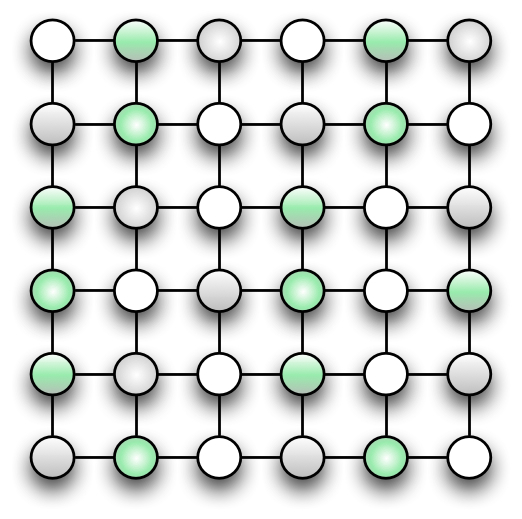
\includegraphics[width=5cm]{gfx/distributed/cellular.jpg}
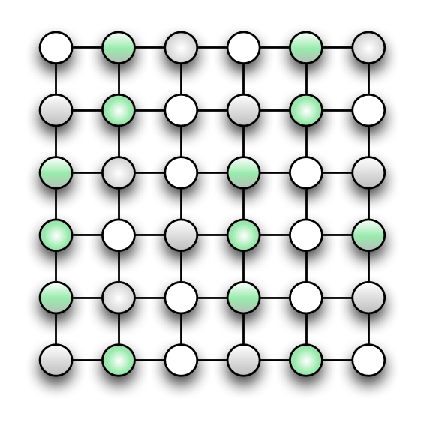
\includegraphics[width=15pc]{cellular.eps}
\caption{Cellular Evolutionary Algorithm.}
\label{fig:cellular}
\end{figure}

\end{description}





%%%%%%%%%%%%%%%%%%%%%%%%%%%%%%%%%%%%%%%%%%%%%%%%%%%%%%%%%%%%%%%%%%%%%%%%%%%%%%%
\section{Massive parallelization on General Purpose GPUs}
\label{sec:parall_and_GPUs}
%%%%%%%%%%%%%%%%%%%%%%%%%%%%%%%%%%%%%%%%%%%%%%%%%%%%%%%%%%%%%%%%%%%%%%%%%%%%%%%

Moore's Law describes a long-term trend in the history of computing
hardware: the number of transistors that can be placed inexpensively
on an integrated circuit has doubled approximately every two
years. The trend has continued for more than half a century and is not
expected to stop, theoretically until not too many years above
2016. On 2005 Gordon Moore stated in an interview that his law cannot
be sustained indefinitely because transistors would eventually reach
the limits of miniaturization at atomic levels. Maybe it is time for
Koomey's Law \cite{10.1109/MAHC.2010.28} to replace Moore's
Law. Koomey says that energy efficiency is doubled every 18
months. For fixed computing load, the amount of battery you need will
fall by a factor of two every year and a half.

Parallel computation has recently become necessary to take full
advantage of the gains allowed by Moore's law. For years, processor
makers consistently delivered increases in clock rates and
instruction-level parallelism, so that single-threaded code is
executed faster on newer processors with no modification. Now, to
manage CPU power dissipation, processor makers favor multi-core chip
designs, and software has to be written in a multi-threaded or
multi-process manner to take full advantage of the new hardware \cite{6307773}.

Graphics processors have rapidly matured over the last years, leaving
behind their roots as fixed function accelerators, and growing into
almost general purpose computational devices for highly parallel
workloads. Some of the earliest academic work about GPUs as
computational devices date back to University of Washington in 2002
\cite{Thompson:2002:UMG:774861.774894} and Stanford in 2004
\cite{Buck:2004:BGS:1015706.1015800}.  % Esto debería ir en la intro - JJ

GPUs are similar to multi-core CPUs but with two main differences,
as can be seen in Figure \ref{fig:cpu-gpu}. Traditionally, CPU
main interest has been fast execution of single threaded code instead
GPUs are made for throughput. CPUs try to improve the execution of a
single instruction stream while GPUs take the opposite route obtaining
benefits from massively threaded streams of instructions and/or
data. The second difference is how threads are scheduled. The
operating system schedule threads over different cores of a CPU in a
preemptive fashion. GPUs have dedicated hardware for the cooperative
scheduling of threads.

\begin{figure*}[!ht]
\centering
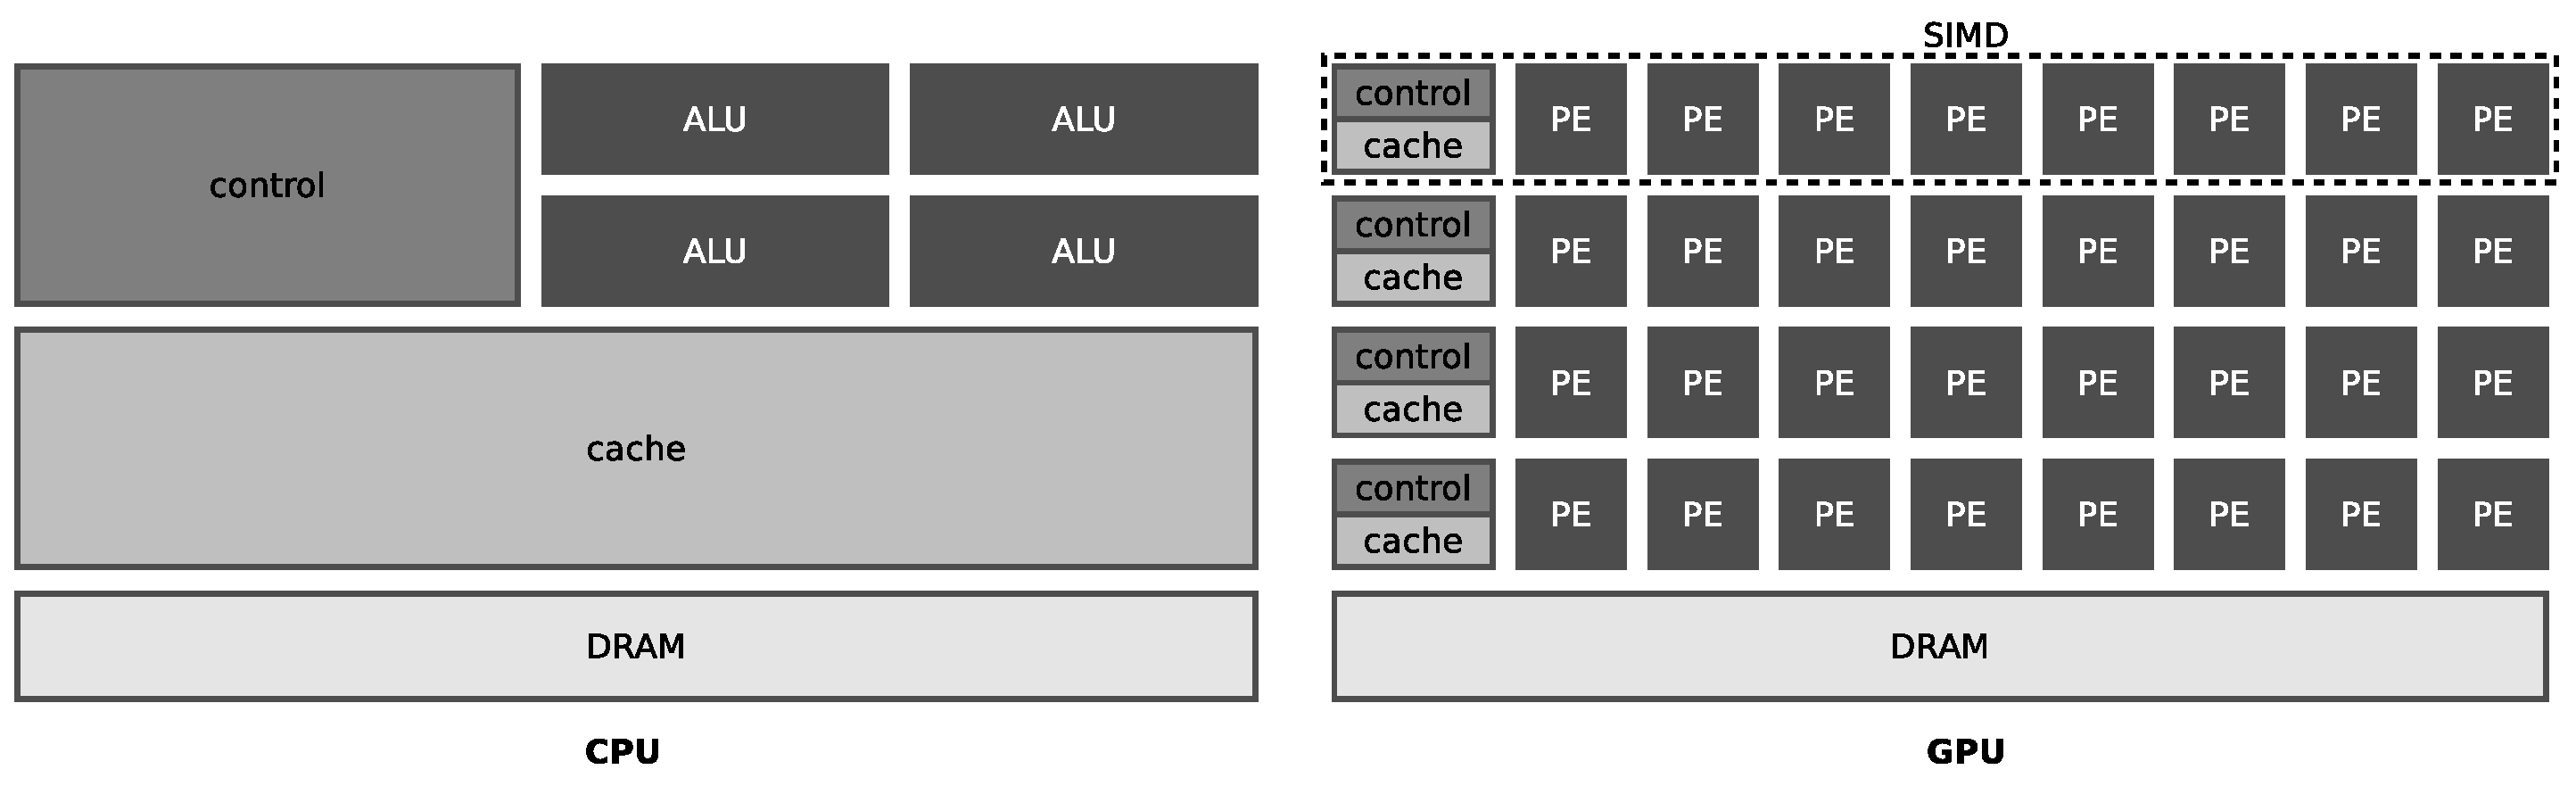
\includegraphics[width=\textwidth]{cpu-gpu.eps}
\caption{CPU and GPU block diagram comparison.}
\label{fig:cpu-gpu}
\end{figure*}

Physically GPUs are huge in comparison with CPUs as shown in Table \ref{tab:features}. Latest microprocessors from the two main vendors, AMD and Intel, are over 1 billion transistors while latest GPUs from AMD and NVIDIA \cite{nvidia} are over 7 billion transistors. CPUs draw 100W at most, a limit established by the cost of commodity heat sinks and fans. GPUs have bigger power consumption and currently can be reach 400 to 500W. This is made possible with the use of exotic cooling solutions. CPUs are built with the finest technology, read best lithography available, while GPUs are made with budget in mind in cheaper processes.

No standard terminology can be found in the world of graphics hardware.
Every company have a  different set of terms to refer to the same
underlying objects and principles. Many authors try to alleviate this
lack of standard terms calling `shader core' to an Intel Execution
Unit (EU), an AMD Single Instruction Multiple Data (SIMD) or an NVIDIA
Streaming Multiprocessors (SM). Any of these refer to a single
processor core inside of the GPU that can fetch, decode, issue and
execute instructions. The shader core is composed of several
execution units (EU) that can execute an individual vector operation
equivalent to an Advanced Vector Extensions (AVX) or Streaming SIMD
Extensions (SSE) instruction. AMD call this kind of EU streaming
processor (SP), while NVIDIA uses the term CUDA core. Table
\ref{tab:features} compares several existing CPUs, GPUs and
Accelerated Processing Units (APUs), taking into account these terms
and their meaning.

\begin{table*}[!ht]
\resizebox{\textwidth}{!}{
\centering
\begin{tabular}{|c|c|c|c|c|c|c|c|c|}
\hline
                       & estimated     & die          & (shader)      & clock rate & memory       & GFLOPS          & TDP & approx.\\
manufacturer \& model  & transistors   & area         & cores         & (GHz)      & bandwidth    & (single         &     & price  \\
                       & (billions)    & ($mm^2$)     & CPU/GPU       & CPU/GPU    & (GB/s)       & precision)      & (W) & (\$)   \\
\hline
\hline
AMD Opteron 6386 SE     & 2.4           & 630          & 16            & 3.5        & 75           & 332.8          & 140 & 1392   \\
\hline
Intel Xeon E7 8890 V4   & 5.69          & 662          & 24            & 2.2        & 102          & 3500           & 165 & 7174   \\
\hline
\hline
AMD A10-7890K           & 2.41          & 245          & 4/512         & 4.1/0.866  & 15.76        & 1018           & 95  & 150    \\
\hline
Intel Core i7 6950X     & 3.2           & 122          & 10            & 3.0        & 34           & 900            & 140 & 1723   \\
\hline
\hline
AMD Radeon RX 480       & 6.2           & 438          & 2304          & 1.266      & 256          & 5100           & 150 & 200    \\
\hline
NVIDIA GeForce GTX 1080 & 7.2           & 314          & 2560          & 1.607      & 320          & 8228           & 180 & 700    \\
\hline
\hline
AMD Radeon R9 290X      & 6.2           & 438          & 2816          & 1          & 320          & 5632           & 250 & 550    \\
\hline
AMD Radeon R9 295X2     & $2\times6.2$  & $2\times438$ & $2\times2816$ & 1.018      & $2\times320$ & $2\times5733$  & 500 & 1500   \\
\hline
AMD Radeon R9 Fury X    & 8.9           & 596          & 4096          & 1.050      & 512          & 8601.6         & 275 & 650    \\
\hline
NVIDIA GeForce GTX 980M & 5.2           & 398          & 2048          & 1.126      & 224.3        & 3189           & 165 & 550    \\
\hline
NVIDIA GeForce Titan Z  & $2\times7.08$ & $2\times561$ & $2\times2880$ & 0.705      & $2\times336.5$ & 8122         & 475 & 1500   \\
\hline
\hline
AMD FirePro S10000      & $2\times4.3$  & $2\times352$ & $2\times1792$ & 0.825      & $2\times240$ & $2\times2956$  & 375 & 3000   \\
\hline
NVIDIA QUADRO K6000     & 7.1           & 561          & 2880          & 0.9        & 288          & 3950           & 225 & 5000   \\
\hline
\hline
NVIDIA Tesla K40        & 7.1           & 561          & 2886          & 0.745      & 288          & 5364           & 235 & 4000   \\
\hline
Intel Xeon Phi 5100P    & 5             & 600          & 60            & 1.053      & 320          & 2020           & 225 & 2200   \\
\hline

\end{tabular}
}
\caption{CPUs, APUs and GPUs comparison of the best professional and commodity desktop hardware available nowadays. A slash is used in APUs to separate CPU/GPU parts. \label{tab:features}}
\end{table*}

% Antonio - TODO: update table with new cards

Nowadays NVIDIA has one of the best performance for GPU computing \cite{benchmarkGPU2015} and in the second step is AMD. Both makers take different compromises in the design of theirs GPUs. AMD has more execution units but its memory hierarchy is weaker. This way software bounded by memory bandwidth or with strong ordering inter-dependencies prefers NVIDIA hardware. On the other side, loads capped by pure ALU execution power use to be faster on AMD hardware.

Traditionally CPUs and GPUs have been separated. In 2016 the trend is
to integrate both into a single chip for cost efficiency reasons. Only
top models remain as discrete devices. Some of this are top models
from Intel's Core i7 or AMD's Opteron 6300 families. Also best
discrete GPUs from NVIDIA and AMD, like consumer GeForce GTX 1080 and
Radeon RX 480 and professional line QUADRO K6000 and Radeon FirePro
S10000.

From 2006 CPUs with an integrated GPU have became popular. AMD and Intel started selling this kind of combined processor and graphics card. The term Accelerated Processing Unit has been coined for this kind of chips. The architectural names are Llano for AMD and Sandy Bridge for Intel. Many reviews state that AMD's CPU cores are slower than Intel's ones but their GPU is faster. Latest Intel APUs, based on Skylake microarchitecture, integrate a more powerful GPU unit with up to 72 cores, Iris Pro Graphics 580. Which combination is better is not an easy question to answer. It must be backed by specific benchmarks, or better, the real application that we want it to run.

Over time the use of GPUs has passed from odd to common in our
systems. Actually, several time consuming processes have been
parallelized inside our operating systems such as web page
rendering. However, the speedup that graphics hardware can bring to us
is not free, as each application to be accelerated must be rewritten
to take full advantage of the GPU.

As CPU makers did some years ago, passing from single core to symmetric multiprocessing system (SMP), and more recently to multi-cores, GPU makers are following the same trend. We can connect more than one graphic card to our computer to improve its GPU capacities or buy a card with 2 graphic chips inside. GPUs are so much powerful than CPUs that even a small cluster of a few GPUs can be faster than classic, and much more expensive, big cluster of computers. First cluster of this kind appear in the scientific literature in 2004 \cite{10.1109/SC.2004.26} with big success. Nowadays, more and more people build small GPU clusters with a couple of mighty graphic cards just to game. Connecting 2, 3 or 4 graphics card is called CrossFire by AMD and Scalable Link Interface (SLI) by NVIDIA.

Most information shown in this and next sections is available from the websites of the respective manufacturer: AMD \cite{amd}, Intel \cite{intel} and NVIDIA \cite{nvidia}.


%%%%%%%%%%%%%%%%%%%%%%%%%%%%%%%%%%%%%%%%%%%%%%%%%%%%%%%%%%%%%%%%%%%%%%%%%%%%%%%
\section{GPUs Programming}
\label{sec:programming}
%%%%%%%%%%%%%%%%%%%%%%%%%%%%%%%%%%%%%%%%%%%%%%%%%%%%%%%%%%%%%%%%%%%%%%%%%%%%%%%

%%%%%%%%%%%%%%%%%%%%%%%%%%%%%%%%%%%%%%%%%%%%%%%%%%%%%%%%%%%%%%%%%%%%%%%%%%%%%%%
\subsection{Programming Model}
%%%%%%%%%%%%%%%%%%%%%%%%%%%%%%%%%%%%%%%%%%%%%%%%%%%%%%%%%%%%%%%%%%%%%%%%%%%%%%%

The way GPUs can be exploited is deeply rooted on its hardware. There exists several APIs: every company has a proprietary one tied to their respective products. This way AMD started with Close to Metal and NVIDIA with CUDA. Over time another standard appear, OpenCL \cite{opencl}.

With respect to the programming tools available for developers, most the Application Program Interfaces (APIs) are based on C-like languages, but having some restrictions to improve the parallel throughput, such as no recursion at all or limited pointers usage. A popular option is the open source compiler LLVM \cite{LLVM} from the University of Illinois.

From 2003 the two main GPU developers, ATI an NVIDIA, started selling hardware solutions that need to be programmed with proprietary APIs. Despite previous work, the first widely supported GPUs were DX10 generation GeForce 8 series from NVIDIA, using the more mature CUDA API. On the other hand, the Radeon series from ATI, were programmed with the Close To Metal API.

Paying attention to operating system vendors, there were efforts in the same direction. Some people at Apple betted on the potential of GPUs and started developing an open API, latter known as OpenCL. In the same time, Microsoft created the DirectCompute API for Windows.

OpenCL aimed to became the OpenGL of heterogeneous computing for parallel applications. It is a cross-platform API with a broad and inclusive approach to parallelism, both in software and in hardware. While explicitly targeting GPUs, it also considers multi-core CPUs and FPGAs. The applications are portable across different hardware platforms, varying performance while keeping functionality and correctness. The first software implementations date back to 2009.

Most companies support OpenCL across their products. Apart from AMD and NVIDIA we can use it on graphic hardware from S3 and VIA. Also IBM has a version of OpenCL for PowerPC and CELL processors. Intel started to offer support from the APU architecture Ivy Bridge and GPUs. Embedded world is also interested in OpenCL. Imagination Technologies offer support for the SGX545 graphics core. As does Samsung with their ARM based microprocessors.

To make life easier for potential users many libraries are appearing. One significant example are STL like extensions for the C++ language. In \cite{doi:10.1137/120903683} we can read a comparison of several modern C++ libraries providing high-level interfaces for programming multi- and many-core architectures on top of CUDA and OpenCL.


%%%%%%%%%%%%%%%%%%%%%%%%%%%%%%%%%%%%%%%%%%%%%%%%%%%%%%%%%%%%%%%%%%%%%%%%%%%%%%%
\subsection{Execution Model}
%%%%%%%%%%%%%%%%%%%%%%%%%%%%%%%%%%%%%%%%%%%%%%%%%%%%%%%%%%%%%%%%%%%%%%%%%%%%%%%

OpenCL, DirectCompute and CUDA are APIs designed for heterogeneous computing with both a host CPU and an optional GPU device. The applications have serial portions, that are executed on the host CPU, and parallel portions, known as \textit{kernels}. The parallel kernels may execute on an OpenCL compatible device, CPU or GPU, but synchronization is enforced between kernels and serial code. OpenCL is distinctly intended to handle both task and data parallel workloads, while CUDA and DirectCompute are primarily focused on data parallelism.

A kernel applies a single stream of instructions to vast quantities of data that are organized as a 1-3 dimensional array (see Figure \ref{figure:grid}). Each piece of data is known as a work-item in OpenCL terminology, and kernels may have hundreds or thousands of work-items. The kernel itself is organized into many work-groups that are relatively limited in size; for example a kernel could have 32K work-items, but 64 work-groups of 512 items each.

Unlike traditional computation, arbitrary communication within a kernel is strongly limited. However, communication and synchronization is generally allowed locally within a {\it work-group}. So work-groups serve two purposes: first, they break up a kernel into manageable chunks, and second, they define a limited scope for communication. 

\begin{figure*}[!ht]
\centering
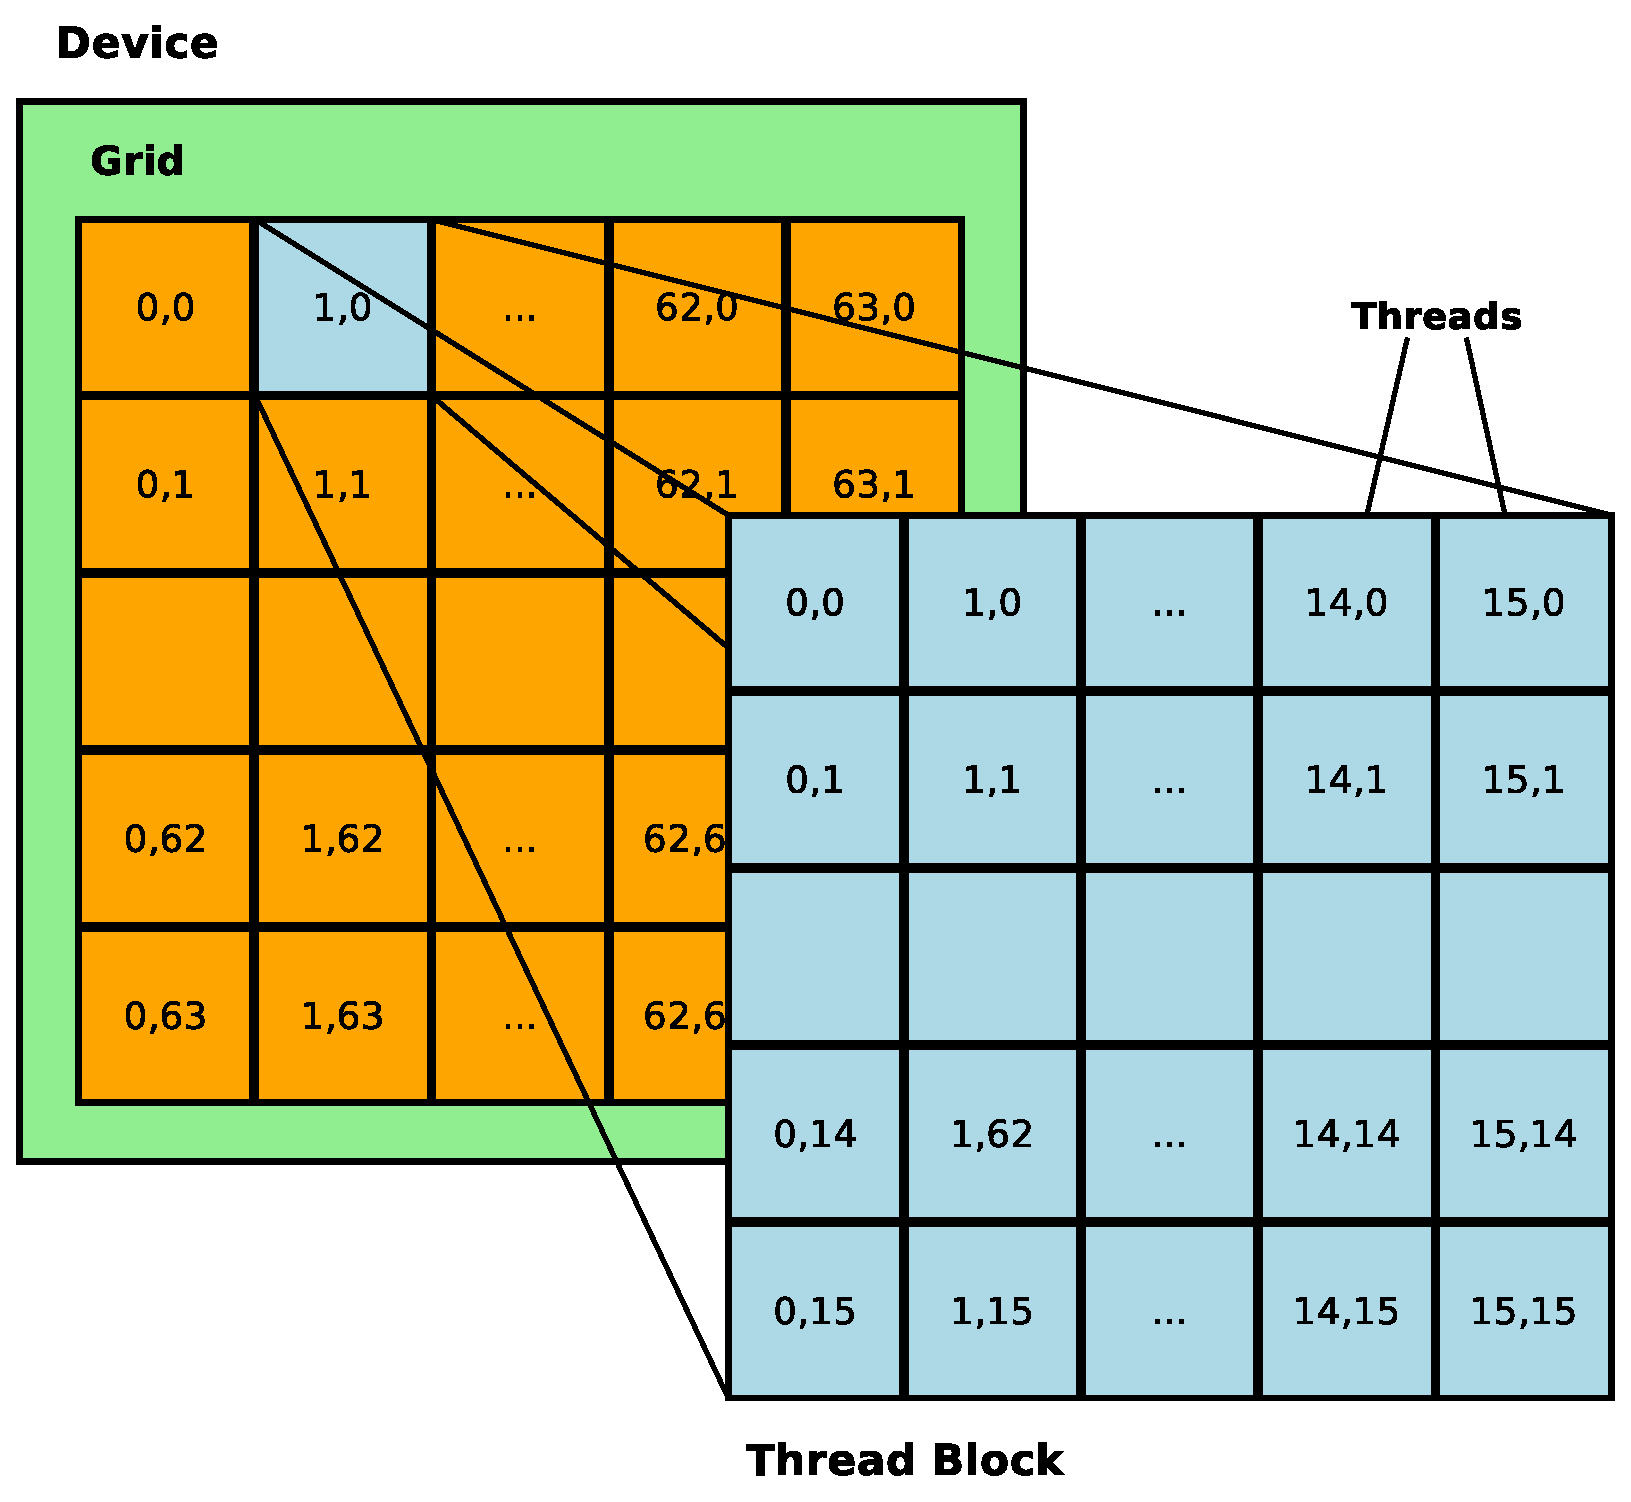
\includegraphics[width=1.0\textwidth]{grid.eps}
\caption{Execution model: Each piece of data is a work-item (thread); a kernel has thousands of work-items and is organized into many work-groups (thread blocks); each work-group process many work-items.}
\label{figure:grid}
\end{figure*}

%%%%%%%%%%%%%%%%%%%%%%%%%%%%%%%%%%%%%%%%%%%%%%%%%%%%%%%%%%%%%%%%%%%%%%%%%%%%%%%
\subsection{Memory Model}
%%%%%%%%%%%%%%%%%%%%%%%%%%%%%%%%%%%%%%%%%%%%%%%%%%%%%%%%%%%%%%%%%%%%%%%%%%%%%%%

The memory model defines how data is stored and communicated within a device and between the device and the CPU. The memory model can be seen in Figure \ref{figure:memory}. DirectCompute, CUDA and OpenCL share the same four memory types but employ different terminology:

\begin{figure*}[!ht]
\centering
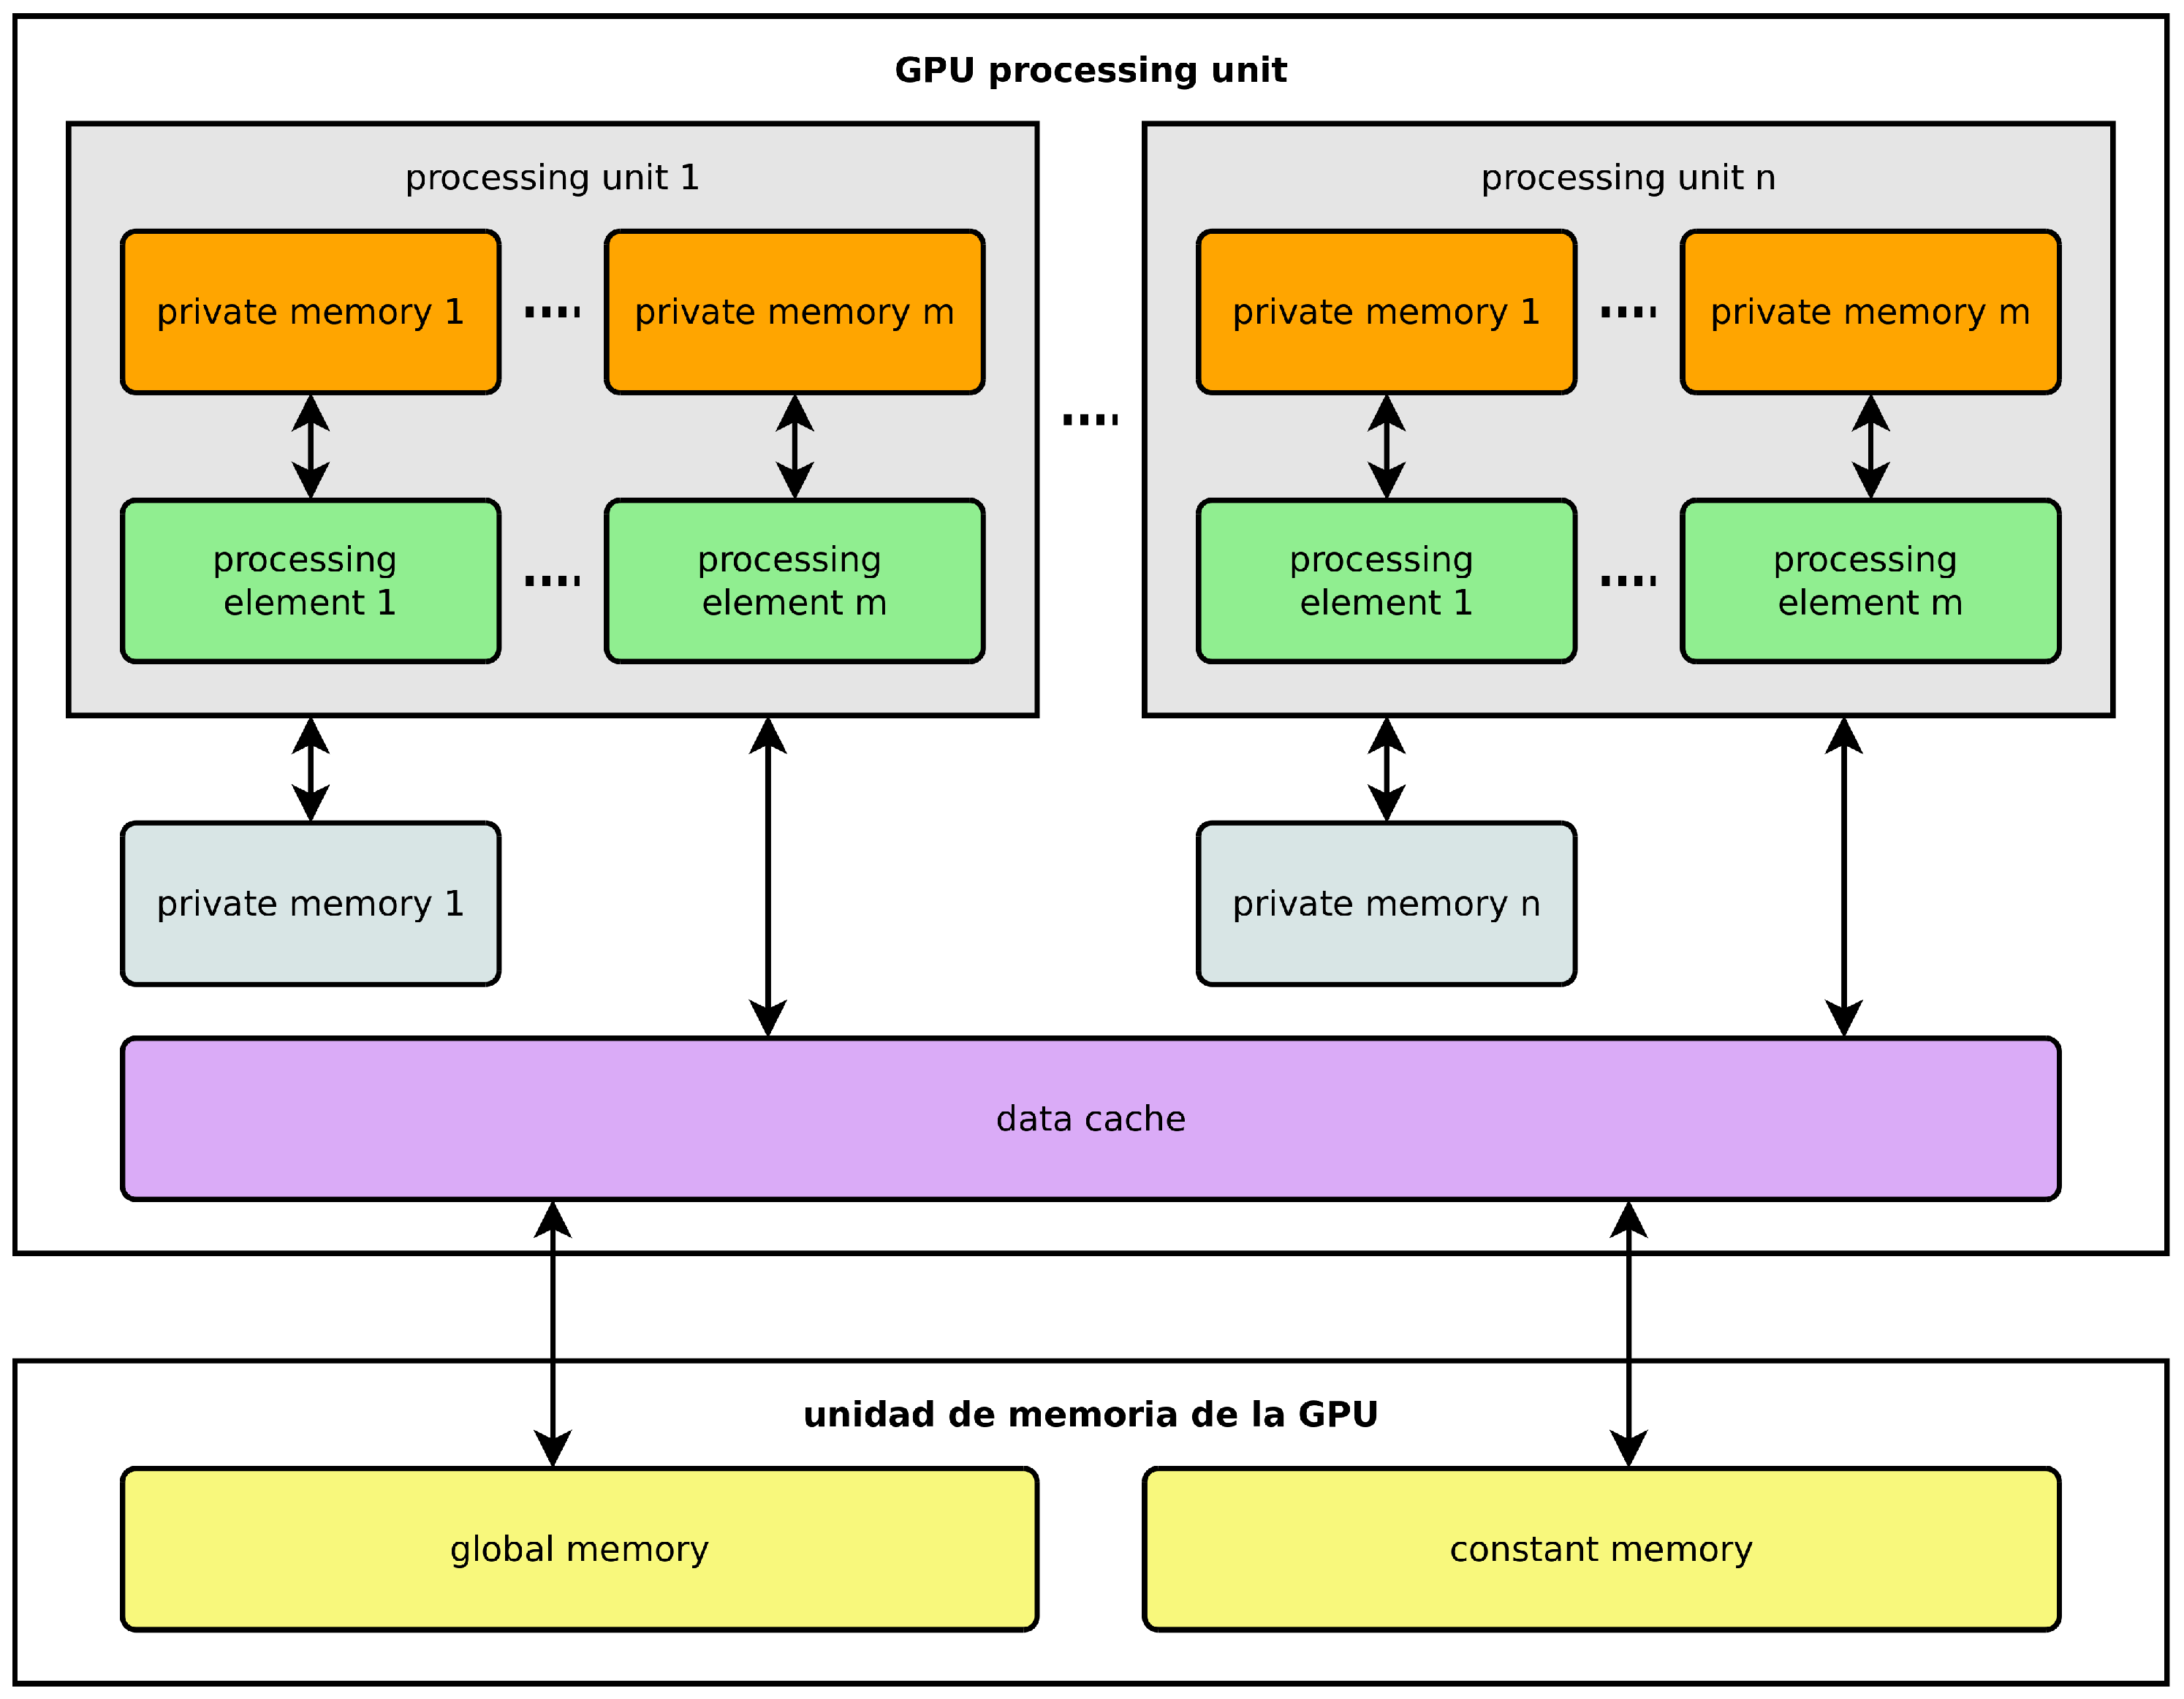
\includegraphics[width=1.0\textwidth]{memory.eps}
\caption{Memory model defines how the data is stored and communicated between CPU and GPU. Global memory is RW for both CPU and work-items; constant memory is RW for CPU and RO for work-items; private memory is RW for a single work-item; local memory is RW for a work-group.}
\label{figure:memory}
\end{figure*}

\begin{itemize}
\item Global memory: it is available for both read and write access to any work-item and the host CPU.
\item Constant memory: is a read-only region for work-items on the GPU device, but the host CPU has full read and write access. Since the region is read-only, it is freely accessible to any work-item.
\item Private memory: is accessible to a single work-item for reads and writes and inaccessible for the CPU host. The vast majority of computation is done using private memory, thus in many ways it is the most critical term of performance.
\item Local memory: is accessible to a single work-group for reads and writes and is inaccessible for the CPU host. It is intended for shared variables and communication between work-items and is shared between a limited number of work-items.
\end{itemize} 

Unfortunately many times we have to pass data from CPU to GPU before a serious calculation can be done. Also after that, CPU must gather results from the GPU. Too much data passing can ruin speedups so they should be minimized if it can't be avoided at all.

These problem have been with us because current CPUs and GPUs have been designed as separate processing elements and do not work together efficiently. At least until last APUs from AMD. New AMD A7 series uses what they call Heterogeneous System Architecture (HSA). HSA seamlessly shares data between CPU and GPU, without memory copies or cache flushes with minimal dispatch overhead. Both components can share a common memory architecture.

Different EAs adapt to the limitations of the memory model with different degrees of success. Talking about population size, the smaller the the better. The variability is huge between different kinds. Also when possible, many small islands is preferable to a big unique population. The same is valid for any aspect of the algorithm which demands a big quantity of memory.


%%%%%%%%%%%%%%%%%%%%%%%%%%%%%%%%%%%%%%%%%%%%%%%%%%%%%%%%%%%%%%%%%%%%%%%%%%%%%%%
\section{Parallelizing EAs on GPGPUs}
%%%%%%%%%%%%%%%%%%%%%%%%%%%%%%%%%%%%%%%%%%%%%%%%%%%%%%%%%%%%%%%%%%%%%%%%%%%%%%%


\subsection{Frameworks used with EAs}

In this section we cite some relevant material not in the EA field but involved with the programming frameworks used to implement EAs in a more convenient way. Most evolutionary metaheuristics can be implemented without effort by using any of the existing frameworks. 

The most complete and comprehensive review of these frameworks is from Parejo \cite{springerlink:10.1007/s00500-011-0754-8}. It is a comparative study of metaheuristic optimization frameworks. As criteria for comparison, a set of 271 features grouped in 30 characteristics and 6 areas has been selected. These features include the different metaheuristic techniques covered, mechanisms for solution encoding, constraint handling, neighborhood specification, hybridization, parallel and distributed computation, software engineering best practices, documentation and user interface. The difference is that this survey just includes frameworks with GPGPU support only for evolutionary computation metaheuristics. 

PUGACE\cite{5586286} is a framework in CUDA for cellular GAs (cGAs), but only for linear neighborhood structures. The architecture of this framework is presented and experiments with the QAP problem are performed. Fitness evaluation uses a thread for each chromosome. Speedups for several problem instances varies from $\times15$ to $\times18$. The execution platform was a Pentium Dual Core at 2.5Ghz and an nVidia GeForce 98000 GTX+.


\subsection{Requirements and constraints to parallelize EAs on GPUs}

% Antonio - TODO: Fill this section with the general features/issues to take into account when parallelizing EAs on GPUs. Try not to overlap with the Taxonomy section.

** The idea here is to describe overall the way to parallelize EAs on GPUs: requirements, issues to consider, constraints that GPUs have (to do this task), etc **


%%%%%%%%%%%%%%%%%%%%%%%%%%%%%%%%%%%%%%%%%%%%%%%%%%%%%%%%%%%%%%%%%%%%%%%%%%%%%%%
\section{Parallelization Taxonomy}
\label{sec:taxonomy}
%%%%%%%%%%%%%%%%%%%%%%%%%%%%%%%%%%%%%%%%%%%%%%%%%%%%%%%%%%%%%%%%%%%%%%%%%%%%%%%

This section proposes a taxonomy to distinguish between the different distribution methods applied in the literature. It is inspired by the classical models used in the distribution of EAs. 
There are many different bioinspired approaches included in the bibliography, but we are mainly focused on Parallel Evolutionary Computation (EC). That is the most extended metaheuristic to address many types of large or complex problems, which require some kind of parallelization to be solved with enough quality and on a reasonable quantity of time.


Alba \cite{Alba2005book} reviewed and surveyed parallel metaheuristics on EC (Evolutionary Computation). They identified the majority of paradigms with respect to parallel/distributed Evolutionary Algorithms (EAs), according to Flynn's taxonomy, under the Multiple Instruction Multiple Data (MIMD) category. This argument has been fairly valid during the last two decades because the most dominant platform for running parallel/distributed EAs were distributed memory architectures, like clusters. However fine-grained EAs deployed on massive parallel processors (MPPs) are resurfacing, due to GPUs architecture gives low cost support for them.

The parallel EAs community has a wide legacy with MIMD architectures and a very little contribution for SIMD systems. This comes in part due to the dominance of MIMD architectures as compared to SIMD ones.

Alba classifies the main parallel metaheuristics models as follows:
\begin{itemize}
\item Parallel Genetic Algorithms \cite{Cantu-Paz98asurvey} %G. Luque, et al..
\item Parallel Genetic Programming \cite{springerlink:10.1023_A:1021873026259}.
\item Parallel Evolution Strategies \cite{Rudolph92parallelapproaches}.
\item Parallel Ant Colony Algorithms \cite{ParallelAntColony}.
\item Parallel Estimation of Distribution Algorithms  \cite{springerlink:10.1007_3_540_32494_1_7}.
\item Parallel Scatter Search \cite{GarciaLopez2003575}.
\item Parallel Variable Neighborhood Search \cite{Garcia_lopez_theparallel}.
\item Parallel Simulated Annealing \cite{Genetic_parallelsimulated} .
\item Parallel Tabu Search \cite{Crainic97towardsa}.
\item Parallel Greedy Randomized Adaptive Search Procedures \cite{Resendeparallelgreedy}.
\item Parallel Hybrid Metaheuristics  \cite{Cotta05e:parallel}. 
\item Parallel MultiObjective Optimization  \cite{Nebro07mocell:a}.
\item Parallel Heterogeneous Metaheuristics  \cite{ANL04}. 
\end{itemize}

Nevertheless, when the research community uses GPGPU, all the EC approaches are parallel, so we revise the bibliography taking in mind how an algorithm has been parallelized using that paradigm, so, for this survey, the specific metaheuristic used in every paper is being placed in a secondary position.  For that reason, we focus the rest of the survey on the different ways for implementation of Parallel Evolutionary Algorithms (PEAs) as Zhang and Zhenming propose in \cite{ZhangImplementationMasterSlave}: master-slave model \cite{man-leung-wong-parallel-2005}, fine-grained model \cite{jian_ming_li_efficient_2007}, coarse-grained model \cite{Maitre:2009:CGP:1569901_1570089} \cite{pospichalParallelGeneticAlgorithOnCUDA2010} or hierarchical models  \cite{DBLP:conf/gecco/PospichalMOSJ11} that use two or more of the previous parallel approaches in an hierarchical way. 


%%%%%%%%%%%%%%%%%%%%%%%%%%%%%%%%%%%%%%%%%%%%%%%%%%%%%%%%%%%%%%%%%%%%%%%%%%%%%%%
\subsection{Taxonomy}
%%%%%%%%%%%%%%%%%%%%%%%%%%%%%%%%%%%%%%%%%%%%%%%%%%%%%%%%%%%%%%%%%%%%%%%%%%%%%%%

The proposed taxonomy is based on the classical approach followed by other authors, but it adds two new groups that we consider important: the hierarchical and the non-standard models.

\subsubsection{Master-slave approaches}
Master-slave Evolutionary Algorithms traditionally solve problems involving computationally expensive fitness functions, where the master node runs the entire algorithm while the slaves execute the fitness evaluation of the individuals. Using this approach, the evaluation of the fitness function is not sequential, but in parallel, so the master-slave version is more efficient because the evaluations usually are the more expensive portion of the total run time.

\subsubsection{Fine-grained approaches}
Cellular Evolutionary Algorithms (CEAs) or Fine-grained Evolutionary Algorithms have not had as much impact as other types of PEAs. The main reason is that they adapt themselves very well to the especial hardware architecture, with shared memory, but very bad to other distributed memory architectures. On the other hand, parallel distributed memory architectures supply all loosely coupled algorithms and the fine-grained EAs are not included into this category. The main reason behind that is the high cost of building massively parallel architectures which normally attracted fewer researchers to work on fine-grained EAs. However, a review of the trends in parallel architectures foresees a strong increase in fine-grained EAs face to face other EA categories. This is due to three reasons: 

\begin{itemize}
\item Growing trend of massive number of processors on chip or card. 
\item The high inter-processors speed which is a major factor affecting the efficiency of fine-grained EAs. 
\item The huge low cost of these architectures which attract a wide base of researchers and developers. 
\end{itemize}

For this category of algorithms, each individual is a parent at the beginning of the algorithm and it looks for the second parent by selection in a neighborhood. As a result CEAs provide automatic niching effect, avoiding an early convergence. 

\subsubsection{Coarse-grained approaches}
These approaches work with a set of sub-populations, normally a part of the whole population, distributed in different nodes, being every node devoted to work with just one of them, so they can work in parallel independently. Each of these sub-populations is known as an `island'. In the standard model, after a number of generations one or more individuals, normally the best, are interchanged, as dictated by migration rate, between islands, which are connected following a specific neighborhood topology.


\subsubsection{Hierarchical models}
This hybrid model just utilizes two or more of the master-slave, coarse-grained and fine-grained approaches in an hierarchical method. At the higher level, an island model algorithm runs while at the lower level, the demes, or sub-populations, are running in parallel, fine-grained, master-slave or even another island model with high migration rates. Hybrid models are not the most common in traditional implementation of EAs due to:
\begin{itemize}
 \item The need for additional parameters related to the more complex topology structure. 
 \item The need for `quite rare' hierarchical parallel architectures to host hybrid algorithms. 
\item The high complexity of programming such models. 
\end{itemize}

Nevertheless, for the GPUs, hybrid EAs are a perfect candidate to exploit the hierarchical memory and flexible block sizing, by means of well structured populations. 


\subsubsection{Non-standard approaches}
By the end of the work we have included a subsection for non-standard approaches \cite{DBLP:conf/gecco/PospichalMOSJ11} including  papers which may not be included in any of the previous ones because they mapped the algorithms and the problem they solve in a special way that cannot be considered as fine grained, coarse grained or master-slave ones.



%%%%%%%%%%%%%%%%%%%%%%%%%%%%%%%%%%%%%%%%%%%%%%%%%%%%%%%%%%%%%%%%%%%%%%%%%%%%%%%
\section{Literature analysis and review} 
\label{sec:survey}
%%%%%%%%%%%%%%%%%%%%%%%%%%%%%%%%%%%%%%%%%%%%%%%%%%%%%%%%%%%%%%%%%%%%%%%%%%%%%%%

In this section we present a quantitative analysis of published papers on EAs on GPUs. Then, the most relevant ones are classified following the previously described taxonomy.

\subsection{Paper gathering} % Gustavo: que te parece este

Firstly, a deep analysis of the existing related literature has been conducted. In order to conduct this analysis we performed the query ``\textit{(GPGPU OR GPU) AND (GENETIC OR EVOLUTIONARY)}'' in the Web Of Science (WoS)\cite{wos} database, referred to any part of the publications, and just enclosed into {\em Computer Science} research area. 
% Antonio - comprobar si se busc� en cualquier parte de los art�culos
We got 320 references, and we eliminated those references unrelated to the scope of this paper (for example, those whose topic is related with genetic engineering and not with genetic algorithms). After that removal, we kept 191 results, which we read in order to extract its features and useful information for this survey.

Looking at the publication rate per year inside this scope, it can be noticed in Figure \ref{figure:publications}, the publication figures has been increased  every year, starting from 2004 (according to the results), being nowadays a field very attractive for researchers and very prolific.

\begin{figure*}[!ht]
\centering
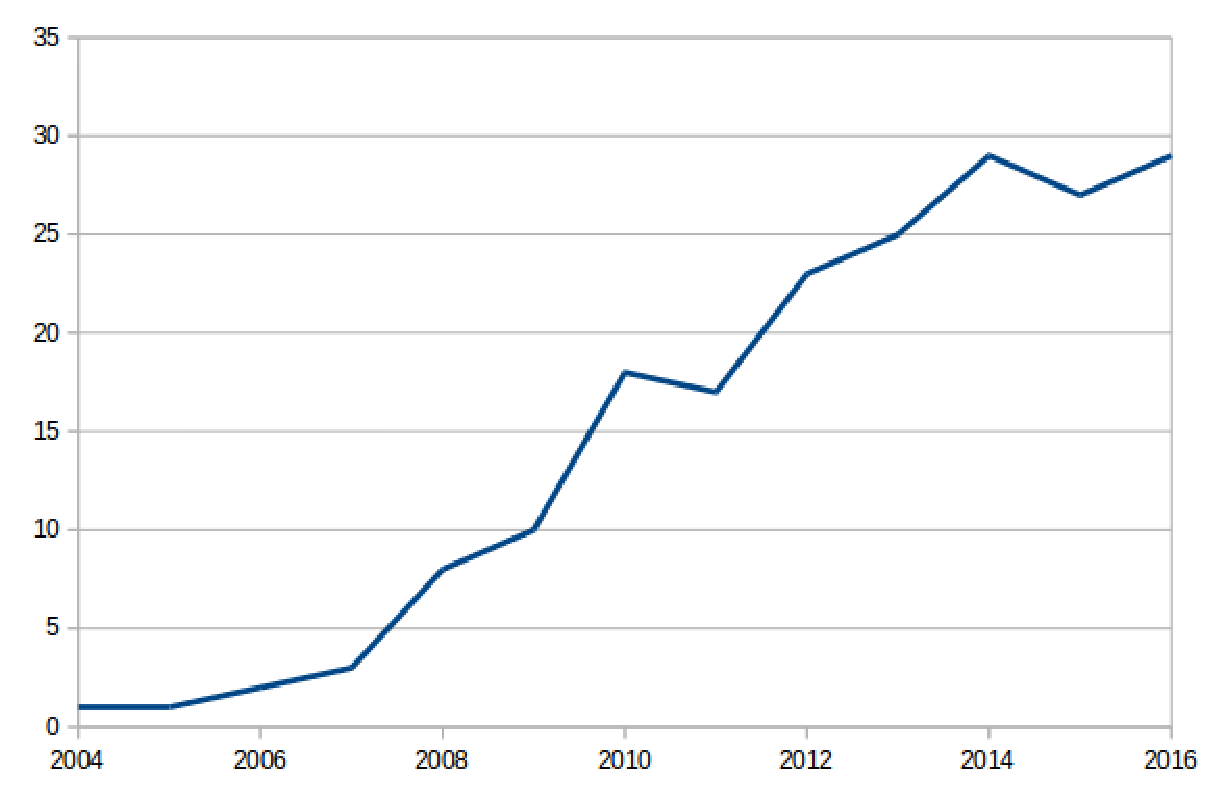
\includegraphics[width=0.9\textwidth]{years.eps}
\caption{Papers published per year inside the scope analyzed here (EAs on GPGPUs) according to Web of Science database.}
\label{figure:publications}
\end{figure*}



With respect to the type of publication, as expected, it can be seen in Figure \ref{figure:type_publication} that conferences and journals share almost all the cake, being slightly higher the figures for conference papers, as it is obviously easier to get published there. However, this factor should be taken just as a reference, since not all the conferences and journals are indexed in WoS, but mainly relevant ones.

\begin{figure*}[!ht]
\centering

\includegraphics[width=0.6\textwidth]{papertype.eps}
\caption{Type of publication, being Conference paper, Journal Paper, or Book Chapter.}
\label{figure:type_publication}
\end{figure*}

Regarding the type of EA implemented or studied in those papers, Figure \ref{figure:type_algorithm} shows the percentages of the different approaches. The most prolific ones are GAs, since it is the classic optimization method inside EAs. It is easy to implement and normally yields very good results.  GP and DE (Differential Evolution) are more specific and thus, less extended or used. `Others' refers to EAs such as EDA (Estimation of Distribution Algorithm), SGS (Systolic Genetic Search) or MA (Memetic Algorithms), to cite a few.

\begin{figure*}[!ht]
\centering
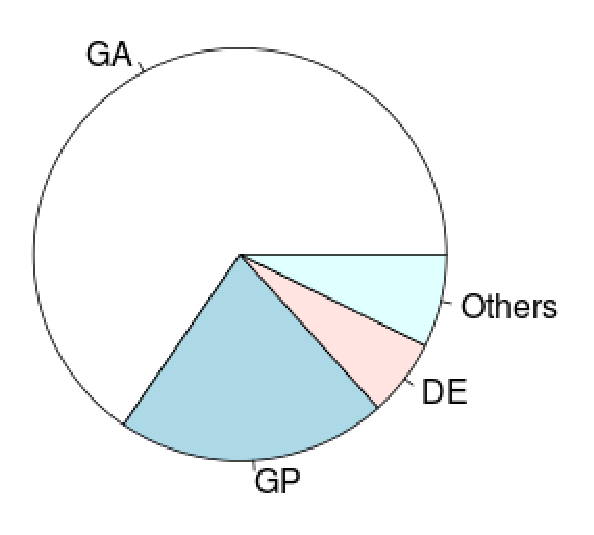
\includegraphics[width=0.6\textwidth]{algorithmtype.eps}
\caption{Type of Evolutionary Algorithm implemented in the analyzed publications.}
\label{figure:type_algorithm}
\end{figure*}

Finally, the majority of the analysed publications deal with solving real problems as it is presented in Figure \ref{figure:type_problem}. This means that the parallelization using GPUs is very effective and can be used in relevant and very hard problems, as real world ones normally are.

\begin{figure*}[!ht]
\centering
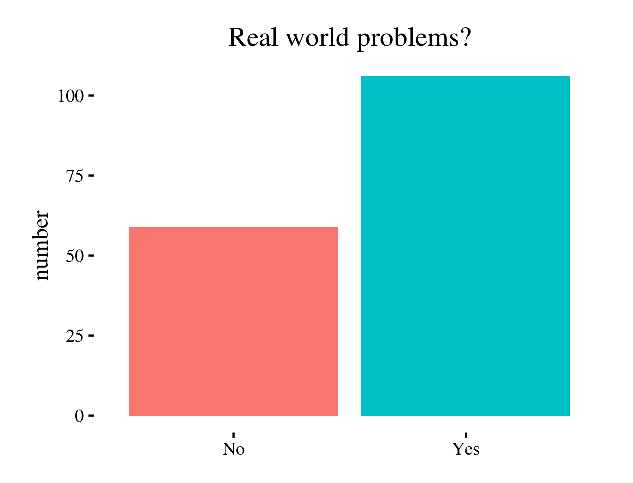
\includegraphics[width=0.6\textwidth]{realproblem.eps}
\caption{Portion of the analyzed publications which address real problems.}
\label{figure:type_problem}
\end{figure*}


Once we have analyzed the whole literature, in the following sections we will go through each of the different groups of the proposed taxonomy. Then, for every one the most representative or relevant works (mainly according to their number of citations) are reviewed and commented.

%After reading this section it is clear than PEAs is an active research field and there are so many different variations that almost for sure one of then can fit the needs of most users. Following this reasoning, in the next 5 sections, the most representative works of every type of EA are going to be presented for your convenience.

%%%%%%%%%%%%%%%%%%%%%%%%%%%%%%%%%%%%%%%%%%%%%%%%%%%%%%%%%%%%%%%%%%%%%%%%%%%%%%%
\subsection{Master-slave Approaches}
\label{sec:masterSlave}
%%%%%%%%%%%%%%%%%%%%%%%%%%%%%%%%%%%%%%%%%%%%%%%%%%%%%%%%%%%%%%%%%%%%%%%%%%%%%%%

As a GPGPU implementation, the GPU is responsible for fitness
evaluation but it does not get involved with other phases of the
algorithm such as crossover, selection or even population ranking for
the next generation. In this approach, every generation the
individuals are copied to the global memory of the GPU, so every
single processor gets one or more individuals from global memory and
puts them into the shared memory, in order to decrease global memory
overhead. After that, each thread evaluates it or them, and stores the
result into the global memory again. Usually each single core
evaluates one individual. The programmer has to minimize the number of
global memory accesses, as well as to minimize data transfers between
CPU and GPU. Some additional problems might be faced, like for
example, individuals that require additional data for being evaluated,
such as a distance matrix or a data set. This additional information
might be copied from CPU to GPU once at the beginning of the process,
so the threads might access this data for evaluation minimizing CPU/GPU 
traffic.

One of the first proposals for parallel Evolutionary Computation using
a GPU was done by Wong et
al. \cite{man-leung-wong-parallel-2005}. They presented an
Evolutionary Programming (EP) algorithm %without crossover EP does not
                                %have crossover - JJ
for solving
five simple test functions, called Fast Evolutionary Programming
(FEP). In this master-slave approach, some actions such as the main loop of the algorithm were executed in
the CPU, while evaluation and mutation were run within the GPU device
because both steps do not need 
of external information exchange. In this case, the reproduction
process implies interaction among, at least, two individuals so the
authors eliminated this step in the algorithm. A maximum speedup of
$\times5.02$ was obtained when the population size increases. This is
the most common organization in GPU implementations, since no
interaction among individuals is required during the evaluation, so
this process can be fully parallelized. In that paper the individuals
was real-coded and the genomes were mapped into the texture
memory. Each GPU thread evaluated one individual and returned its
fitness at the end of the parallel process to the CPU, for the next
evolution cycle. 

A Genetic Programming (GP) method proposed by Harding and Banzhaf \cite{4215552} uses the GPU only for performing the evaluation, while the rest of the steps of the algorithm are run on the CPU. The authors tested real-coded expressions in up to 10000 nodes, boolean expressions in up to 1500 nodes, and some real world problem where they evaluate expressions in up to 10000 nodes. In some cases, the results yielded speedup of thousand times.

Zhang et al. \cite{ZhangImplementationMasterSlave} adapt different EAs to a GPU using CUDA. The authors implemented an hierarchical parallel genetic algorithm using a deme model at high level, and a master-slave schema at low level. In this implementation, the CPU initializes the populations and distributes them to thread blocks in shared memory. Then, GPU threads within each block run a GA independently, selection, crossover, mutation and evaluation, and migrates individuals to other thread blocks in its neighborhood. In this case, no speedup results were reported.

Van Luong et al. \cite{5586403} published in 2010 a methodology for mapping the search space onto the GPU memory hierarchy in three levels: the distribution of the search process among the CPU and GPU (1), the mapping of the neighborhood in the GPU threads (2), and the effective usage of the texture memory in the context of hybrid EAs (3). Experiments to solve the QAP problem with CUDA were presented, where the evolutionary process was performed in the CPU and the generation of the Local Search neighborhood are performed on parallel in the GPU, achieving an acceleration of $\times14.6$ times faster. Hardware used was Core 2 Duo 2,67 Ghz and Nvidia GTX 280. As it can be seen this work also showed the benefits of using a conjunction of CPU and GPU, being the GPU used only for intensive calculations.

There are other papers related with the previous approach, like the one by Tsutsui et al. \cite{Tsutsui:2011:GECCO}. This work uses a master-slave approach with an Ant Colony Optimization (ACO) algorithm \cite{Dorigo:1999:ACO:329055.329062} and Tabu Search \cite{Glover:1997:TS:549765}. Tsutsui uses an Intel Core i7 965 (3.2 GHz) processor and a single NVIDIA GeForce GTX480 GPU. They compare CPU and GPU implementations with and the results showed that GPU computation with MATA, an efficient method for thread assignment cost which they call Move-Cost Adjusted Thread Assignment, showed a promising speedup compared to computation with CPU.

There are papers related with other subjects % cuales subjects? - JJ
like \cite{Pedemonte:2011:BOG:2001858.2002031} which studies the impact of using different representations for binary problems in GPUs to evaluate GAs: boolean data type versus packing multiple bits in a non-boolean data type. The execution platform was a PC with Quad Core Intel Xeon E5530 processor at 2,4 Ghz and a Tesla C1060 with 240 CUDA cores. The CPU only calculates the initial population and a matrix of random number to be used in crossover and mutation by the GPU. The authors review the problem of the data types when GPGPU is used. Several data types of 8, 16, 32, and 64 bits are compared in CPU and GPU versions. Results shows that
packing in 32 bits data types achieve speedup values of up to
$\times100$ compared with boolean data types, specially when the size
of the instances increases. This make sense because the Tesla C1060
are equipped with 32-bit integer ALUs.  

Cano et al. \cite{SpeedingTheEvaluationofGPCano:2012} described a massively parallel evaluation model using a Genetic Programming algorithm for evolving rules for dataset classification. They copied the dataset to the GPU global memory, and evaluated the rules (individuals) for each instance of the dataset in parallel (match kernel). At the end, each successful match was reduced getting each individual fitness (reduction kernel). The implementation, based on CUDA, speedups the fitness calculation phase and greatly reduce the computation time. Results were compared using one, two and four CPU threads and the combination of one or two GPUs of different features (285 cores for GPUa -NVIDIA GeForce 285 GTX- or 480 cores for GPUb -NVIDIA GeForce 480 GTX-). They test three classification algorithms and the results were not very significant for small datasets, but they increased the speedup with large datasets until $\times820$ using two GPUs with 480 cores each one.

The work by Chitty \cite{Chitty16FastParallel} uses a Master-Slave architecture for evaluating at time the population for four GP problems. The results were achieved using an NVidia GeForce Kepler 670 GTX graphics card and compared with a previous one-dimensional stack approach for the same problems. The author fit the algorithm until to observe a peak computational speed of over 55 billion Genetic Programming Operations per second a twofold improvement over the previous one-dimensional stack approach.


Recent works are currently being applied to real-world problems. Jaros et al. \cite{Jaros14Wormhole} use GPUs to lower the run time and improve the quality of the solutions in the problem of wormhole switching in collective communications. The start from an evolutionary tool capable of finding optimal communication schedules for various communication patterns on wide range of interconnection networks topologies of up to 256 nodes. The tool consumes tens of hours so they decide to improve it. As the fitness evaluation was responsible for the 93\% of the execution time this was the only part moved to the GPU. In a first step only one GPU was used with speedups up to $\times5$. After that they made a new implementation capable of using 8 GPUs and 30 times faster than the original.

In \cite{Contreras:2012:UGA:2150467.2150469} the authors use a CPU-GPU architecture for stock market trading. The proposed architecture offers the benefices of GPU distribution for stock market researchers, rather for computer architecture experts. The authors used Jacket \cite{jacket:Matlab}, a software platform for the rapid development of GPGPU computing applications within the MATLAB computing environment, C, and C++. However, this framework is no longer available \footnote{\url{http://blog.accelereyes.com/blog/2012/12/12/exciting-updates-from-accelereyes/}}. Steps and guidelines to migrate from CPU code to GPU code are explained, what is a great contribution, because usually, the authors do not include this information in the papers. The algorithm run in the CPU, but all  {\em for} loops in selection, evaluation, crossover and mutation are translated to Jacket's {\em gfor} to be parallelized in the GPU. Three different CPU configurations are used for the experiments: Pentium 4, Pentium SU41000 and Intel Core i7-860. The former is also combined with an nVidia 460GTX for GPU experiments. Different population size are also tested. The time is reduced to 65\% in comparison with the CPU version. Other conclusions are obtained: speedups with high number of individuals, rather than increasing the number of evaluations; and time reduction for  tournament selection  over roulette-wheel selection.

Stock market trading analysis haas also been recently addressed by using GP in GPUs. The algorithm described in the work by Sungjoo et al. \cite{Sungjoo15fastknowledge} is used to solve the problem of knowledge discovery in stock market time series, i.e. finding the so-called precursor patterns, which model events occurred in the time series. Thus, every individual (tree) in the GP algorithm is a pattern, which must be contrasted against the whole dataset to find out if it is a precursor. This is what the evaluation function does. The time series is divided into different subsets, and stored in several GPUs. The data is then copied once and just the new individuals to evaluate and the partial results of the evaluation must be transferred and updated. The run is conducted for 50 generations and with 500 individuals of a maximum depth of 3 levels, using a i7-3820 CPU and 8 CUDA GPUs (GeForce GTX 690). The authors considered 512 threads per block, 260 blocks per grid and just one grid per GPU. The comparison in performance yields a reduction of 56 times for just one GPU to 277 using all of them. This improvement is got using local memory allocation, using the shared memory of blocks instead yields a smaller improvement of around 188 times faster in the best case. Regarding the influence of individuals' tree size (number of nodes) in the performance, the authors show that the running time grows for just one GPU, but when more than four are used, this growing is minimum and could be assumed in order to improve the quality of the results.


%%%%%%%%%%%%%%%%%%%%%%%%%%%%%%%%%%%%%%%%%%%%%%%%%%%%%%%%%%%%%%%%%%%%%%%%%%%%%%%
\subsection{Fine-grained Approaches}
%%%%%%%%%%%%%%%%%%%%%%%%%%%%%%%%%%%%%%%%%%%%%%%%%%%%%%%%%%%%%%%%%%%%%%%%%%%%%%%

Researchers implement fine-grained algorithms using GPGPU, making every scalar processor (SP) to evolve an individual. This individual interacts with other SPs that belongs to the same Streaming Multiprocessor (SM) to perform the basic operations of the algorithm like crossover or mutation. In this approach a big part of the algorithm runs within the GPU and not only the evaluation phase like in previous section (\ref{sec:masterSlave}). The GPU architecture assists the neighborhoods emerge since each group of SMs have a shared memory, where SPs access without penalty. The exchange of information between individuals through this shared memory is inexpensive. However, programmers have to be careful with the information exchange between individuals in different SMs. 

The second problem of this approach is the random number generator. The CPU can easily generate random numbers, but the GPU is not designed for this task. So researchers have to think about how to solve this problem. Usually the algorithm's implementation generate at the beginning a big set of random numbers and they are copied to the GPU as a list. After that, the GPU uses the random list when needed and when it need. This approach saves time for random generation but the list of random numbers has to be limited. Moreover, all SPs could use the random numbers, so the list must be available for every thread. 


Yu et al. \cite{yu-parallel-2005} implemented the first real cellular EA using GPU, for solving the Colville problem \cite{Ng:2005:DFF:1064290.1064296} in 2005. They place the population in a toroidal 2D grid and use the classical Von Newmann neighborhood structure with five cells. They store chromosomes and their fitness values in texture memory on the graphic card, and both, fitness evaluation and genetic operations, are implemented entirely with fragment programs executed in parallel on GPU. Real-coded individuals was represented as a set of 2D texture maps. BLX-$\alpha$ crossover and non-uniform mutation was developed as tiny programs on every pixel at each step in a SIMD-like fashion. They solved some optimization problems and reached a speedup of $\times15$ with a population of 512x512 individuals. They store a set of random numbers at the beginning of the evolution process to solve the random number generation problem when using GPU processors. 

In 2006, \cite{man-leung-wong-parallel-2006} proposed a parallel hybrid GA (HGA) where the whole evolutionary process run on the GPU, and only the random number generation is done in CPU. Every individual is assigned to a GPU thread, and each one selects probabilistically an individual in its neighborhood to mate with it. Just one offspring individual is generated each time, and it replaces the old one in that GPU thread. The authors compare their implementation with a standard GA run in a CPU and the FEP \cite{man-leung-wong-parallel-2005} algorithm. Using a new pseudo-deterministic selection method, the amount of random numbers transferred from the CPU is reduced. HGA reaches speedup of $\times5.30$ when compared against the sequential version. In 2009 Wong et al. \cite{wong-implementation-2009} provide implementation details for fine-grained evolutionary algorithms.  

Liu and Luo \cite{zhongwen-luo-cellular-2006} implemented a cellular algorithm on GPU to solve three different satisfiability problems (SAT) 
using a greedy local search (GSAT) \cite{Selman93domain-independentextensions} and a cellular GA (cGA). 
They saved local minimums using a random walk strategy, jumping to other search space location. 
The cellular GA adopts a 2D toroidal grid, using the Moore neighborhood, stored on texture GPU memory. This implementation generates the random numbers in the GPU (using a generated seed on the CPU at the beginning of the process). They carried out the experiments using two GSAT implementations, CGSAT (with crossover and without mutation) and PGSAT (without crossover and with mutation) running them on CPU and GPU with different population sizes. A great time reduction was reached using the GPU parallelization approach (from 95ms to 18 ms for CGSAT and from 464ms to 77 ms for PGSAT).

Li et al. \cite{jian_ming_li_efficient_2007} proposed a cellular algorithm on GPU for solving some common approximation functions. The authors reported experiments using big populations (up to 10000 individuals) reaching speedups of $\times73.6$ for some implementations. The novelty of this paper is the bit dataset because it is not easy to deal with bit datasets using a GPU due to the memory size restrictions. The GPUs does not support binary operations, but in this paper the authors dealt with binary individuals of 24 bits  and simulated bit-operator by judging each bit of a binary value is 1 or 0. They faced a general problem for all GPGPU community with bit operations. They proposed to use random-textures for random numbers generation, but the random numbers were generated on CPU previously. 

In \cite{Li:2009:PIA:1726585.1726930} the authors proposed an Fine-grained parallel immune algorithm (FGIA) which is an Artificial Immune System combined with evolutionary algorithm to generate several optimization algorithms. They solve three medium-size instances of the Travelling Salesman problem (TSP) using a fine-grained parallel algorithm with CUDA C. The paper enlarges the population size of FGIA and maintains better population diversity. In conclusion, they included a sub-linear relation between the population size and the execution time, which made the proposal very useful for solving difficult problems that require huge population sizes.

Gonz\'alez et al. \cite{springerlink:10.1007978-3-642-12538-619} use CUDA and store individuals and their fitness values in the GPU global memory. Both, fitness evaluation and genetic operators, run on GPU (no CPU is used). 
They use a pseudo random number generator provided by the SDK of CUDA named Merseinne Twister. Their experiments include some general discrete and continuous optimization problems, and they compare physical efficiency and numerical efficacy with respect to CPU implementation. 

Depending on the problem size, fine-grained approaches may improve the efficiency with respect to the coarse-grained version. For example, in the work of Franco et al. \cite{Franco15LargeScale}, two different approaches for strategies for GPU implementations of the evaluation stage of evolutionary rule learning are analyzed and the types of problems where each method performs best have been identified. The coarse-grained implementation is more conservative and only parallelizes the evaluation of instances, while the fine-grained implementation expands the parallelism to the attribute dimension and is faster on data sets with 10 to 50 discrete attributes.


%%%%%%%%%%%%%%%%%%%%%%%%%%%%%%%%%%%%%%%%%%%%%%%%%%%%%%%%%%%%%%%%%%%%%%%%%%%%%%%
\subsection{Coarse-grained Approaches (island model)}
%%%%%%%%%%%%%%%%%%%%%%%%%%%%%%%%%%%%%%%%%%%%%%%%%%%%%%%%%%%%%%%%%%%%%%%%%%%%%%%

Coarse grained algorithms are the most common among parallel EAs. Generally, these algorithms require less tightly coupled parallel architectures, as compared to fine-grained. Coarse-grained EAs divide the main population into sub-populations (also known as islands) which evolve concurrently. This basic feature of coarse-grained EAs hits a physical limit of GPUs. 

In order to run a coarse-grained EA using a GPU, several kernels are run simultaneously, where each kernel handles a sub-population. GPU architecture is not designed to work this way. This limitation of GPU would mean the conventional mechanics of coarse-grained EAs would need to be changed if GPU would be used.

With regard to this topology, one of the first island models on GPU approaches was published on the GPU competition of GECCO 2009 \cite{gecco2009CompetitionPospichal}. It presented some technical details of an island model entirely hard-coded on GPU, with a ring-neighborhood topology. Nevertheless, the evolutionary operators implemented on GPU were only specific to the GECCO competition, and the validity of the experiments is not clear, since the approach just worked on a small number of problems.

Tsutsui and Noriyuki \cite{1570355} propose run a coarse-grained GA on GPU to solve the QAP problem using CUDA. This is one of the hardest optimization problems in permutation domains. 
Their model generates the initial population on CPU and copied it to the GPU VRAM; then, each subpopulation in a GPU (NVIDIA GeForce GTX285) is evolved. At some generations, individuals in subpopulations are shuffled through the GPU VRAM. Results show a speedup from $\times3$ to $\times12$ (using eight QAP instances), in the comparison with an Intel i7 965 processor. 

The model by \cite{LUONG:2010:INRIA-00520464:1} is based on a re-design of the island model.
Three different schemes are proposed: The first one implements a coarse-grained EA using a master-slave model to run the evaluation step on GPU. The second one distributes the EA population on GPUs, while the third proposal extends the second one using fast on-chip memory. 
Second and third approaches reduce the CPU-GPU memory latency, although their parameters (number of islands, migration topology, frequency, and number of migrants) must be adapted to the GPU features. 
Sequential and parallel implementations are compared, obtaining a speedup of $\times1757$ using the third approach.

Pospichal et al. \cite{pospichalParallelGeneticAlgorithOnCUDA2010,9253} propose a parallel GA with island model running on GPU. The authors map threads to individuals, thus, threads-individuals can be synchronized easily in order to maintain data consistency, and on-chip hardware scheduler can swiftly swap existing islands between multiprocessors to hide memory latency. Fast, shared memory within the multiprocessor is used to maintain populations.
Since the population size is limited to 16KB per island on most GPUs, if the population is larger, slower main memory has to be used. The migration process is based on an asynchronous unidirectional ring that requires an inter-island communication (slower main memory has to be used). The authors report speedups up to $\times7000$ times higher on GPU compared to CPU sequential version of the algorithm.


%%%%%%%%%%%%%%%%%%%%%%%%%%%%%%%%%%%%%%%%%%%%%%%%%%%%%%%%%%%%%%%%%%%%%%%%%%%%%%%
\subsection{Hierarchical Models}
%%%%%%%%%%%%%%%%%%%%%%%%%%%%%%%%%%%%%%%%%%%%%%%%%%%%%%%%%%%%%%%%%%%%%%%%%%%%%%%


The design and implementation of a hybrid EA with local search to solve MAX-SAT over GPUs was thoroughly discussed in \cite{Munawar:2009:HGA:1666141_1666143}. Manuwar et al. uses a hierarchical algorithm of 2D structured sub-populations arranged as islands in a 2D grid. Therefore, every individual has 4 neighboring individuals (north, south, east and west) and each sub-population has 4 neighboring sub-populations (north, south, east and west). Instead of using a conventional algorithm for migration between the sub-populations, they introduced a new technique called diffusion. Diffusion is more suitable for implementation of cGAs based pGA over a GPU. In the proposed implementation, the host processor (CPU) acts as a controller while an NVIDIA Tesla C1060 GPU provides the required computational resources. Configuration, memory allocation and initialization are performed over the host processor. After the initialization stage, data is transferred to the device and the code enters a loop. The loop keeps on repeating until the maximum number of generation criteria is satisfied. Results were collected over a system with NVIDIA Tesla C1060 GPU mounted on a motherboard with Intel Core i7 920@2.67GHz as the host CPU. C1060 have 4GB of device memory, 30 streaming multiprocessors, and the total number of processing cores is 240. The maximum amount of shared memory per block is 16KB and clock rate is 1.30GHz. They compare the results of the algorithms over NVIDIA with optimized for local search, mutation, recombination, selection and diffusion (migration) with different implementations using serial implementation, OpenMP implementation over Intel and over Ultra Spark architectures. The found that the maximum speedup is for larger problems, and it is up to $\times25$ if compared the serial implementation over Intel Core 2 Duo 3.3GHz with the NVIDIA implementation. 

Diego et al. \cite{fjdiego-vrp}proposed a parallel strategy for solving the Capacitated Vehicle Routing Problem (CVRP) by means of an ACO algorithm. They combined the CPU processing, random number generation and centralized pheromone information dealing, with the GPU parallel capabilities: initialization of trails, build solutions, choosing of the best solution, and pheromone evaporation. The experiments were conducted on a GeForce GTX460 in a Pentium Dual Core 2.7GHz with 2GB RAM, using CUDA. The results showed a speedup of $\times12$ in the best case.

Delevacq et al. \cite{ACO-on-GPU_Develacq} tests different parallel strategies for the ACO metaheuristic on a NVIDIA Fermi C2050 GPU, on a four-core Xeon E5640 @2.6 GHz with 24GB RAM. The Max-Min Ant System is considered for solving the Travelling Salesman Problem (TSP) for problem sizes of up to 2100 cities. Authors proposed multi-ant (one colony) and multi-colony approaches implemented with CUDA. They distributed the solutions on the GPU processing elements: an ant per thread, and an ant per block respectively. The common structures, pheromone matrix, distances and candidate lists, are stored in shared memory, meanwhile the CPU is used for a preliminary set of random numbers generation and centralized control tasks. For the multi-colony algorithms, a set of ants is assigned to every processing element. This time, almost the whole algorithm is run in the GPU. They obtained speedups of up to $\times19$ in the multi-ant, and up to 8 in the multi-colony approaches, having similar solution quality than the original sequential approach.

Cecilia et al. \cite{Cecilia201342} proposed three different techniques for improving the classical ACO algorithms parallelization on GPUs: a data parallelism scheme for tour construction on GPU, a GPU-based pheromone updating stage, and a roulette wheel implementation on GPU, called I-Roulette. They introduced the queen ants, associated with CUDA blocks, and the worker ants, associated to CUDA threads. The experiments were performed on a four-core Intel Xeon E5620 running at 2.4 GHz, with 16GB RAM, and a NVIDIA Tesla C2050 Fermi. The proposed techniques lead to obtain a speedup factor of up to $\times20$ in comparison with the sequential implementation.

In \cite{5586530} three cellular GA versions are compared: a CPU, a mono-GPU and a multi-GPU version, being the first work in use multi-GPU for cEAs. A 2D grid population is used and divided in two GPUs in the multi version. Selection, recombination, mutation and evaluation are performed in parallel. In the multi GPU case, a thread for each GPU is controlled by a CPU thread and borderline individuals of the sub-populations are exchanged. The speedup ranges from $\times8$ to $\times711$. However, there is not significantly difference between mono and multi GPU versions, probably due the overhead of the CPU. Hardware used is Intel Quad processor 2.67GHz and Nvidia GeForce GTX 285.

During 2012, Luong \cite{luongMetaheuristicsPpsn2012} implemented a GPGPU algorithm from the metaheuristic point of view. In the paper a guideline to exploit heterogeneous computing resources, including GPU and CPUs, for effective hybrid metaheuristics was proposed. The goal of this paper is not the evaluation of the fitness of some individuals, but the parallelization of metaheuristics which were not inherently parallel, like local search algorithms. Task distribution is clearly defined into the paper, the CPU manages the whole sequential Local Search process and the GPU is dedicated to the costly part i.e. the parallel generation and evaluation of the neighbor solutions.

Authors mapped the population to the GPU and applied the parallel metaheuristic to each individual using its neighborhood structure taking advantage of the blocks of threads present in the GPU architecture. The parallelization of these metaheuristics generated several different individuals that the GPU evaluated at the same time. The critical issue was finding efficient mappings between a GPU thread and a particular neighbor. Indeed, this step is crucial in the design of new large neighborhood local search algorithms for binary problems since it is clearly identified as the gateway between a GPU process and a candidate neighbor. They reviewed neighborhoods based on a Hamming distance of one, two and three, and applied their suggestions to Permuted Perceptron problem \cite{KnudsenPermutedPerceptronProblem1999}. They considered a Tabu Search algorithm \cite{TaillardTabySearch1991} using CUDA for each neigborhood with a configuration of Intel Core 2 Duo 2.67GHz with a NVIDIA GTX 280 card. The CUDA implementation increased the number of successful solutions drastically every instance of the problem. Regarding execution time, acceleration factors using GPU are very significant (from $\times24.2$ to $\times25.8$).

In 2014,  \cite{Wang14heterogeneous} used a supercomputer platform to run a CPU+GPU high performance EA. 16 islands of 8 individuals were set as parameters. The experiments were carried in a combination of Intel Xeon X5650 @2.66GHz and  Intel Xeon X7550 @2.0GHz processors, although the paper do not includes information about the graphic cards used. Several instances of heterogeneous scheduling problems were used to compared with other metaheuristics, obtaining better makespans. 


%%%%%%%%%%%%%%%%%%%%%%%%%%%%%%%%%%%%%%%%%%%%%%%%%%%%%%%%%%%%%%%%%%%%%%%%%%%%%%%
\subsection{Non-standard Approaches}
%%%%%%%%%%%%%%%%%%%%%%%%%%%%%%%%%%%%%%%%%%%%%%%%%%%%%%%%%%%%%%%%%%%%%%%%%%%%%%%

Pospichal et al. in 2011 has presented several papers related with GPU devices. One of the last is \cite{DBLP:conf/gecco/PospichalMOSJ11} where they propose to use a GPU device for Grammatical Evolution, evolving complete programs in an arbitrary language using variable length binary strings. For this problem, every individual is a program, so it must be compiled and sent to the GPU for being evaluated every generation. However the most time-consuming part of this approach is to sent the individuals to the GPU and not the evaluation itself, so, the authors propose to evolve the whole Grammatical Evolution algorithm on the GPU with a special mapping function. They mapped one individual per block of threads and one thread is used to manage each individual. They compare the execution time of an Intel Core i7 with NVIDIA GTX 480 using CUDA (CPU implementation with C) an a Java library called GEVA \cite{O'Neill:2008:GGE:1527063.1527066}, which is an interpreted language (CPU implementation using GEVA).  The authors include results for both implementations (C and GEVA) and one GPU implementation, and they compare them with and without overhead for CPU-GPU communication. We include only the results with overhead, because the parallel version needs the CPU-GPU communication, so the authors might take care about it. The results of GPU implementation are in average 5.3 speedup than CPU with C implementation which is an expected result. The speedup grows until $\times102.8$ when GPU implementation and CPU implementation with GEVA are analysed, but the authors do not include any standard deviation results, so we do not consider the last result as the most important of the paper. Thus, this paper proposes two levels of parallelism: 1) individuals are evaluated in parallel (by threads in the same block); and 2) data within individuals (genes, crossover points, mutations, fitness points, etc.) are maintained by parallel access as well (by block of threads).


%%%%%%%%%%%%%%%%%%%%%%%%%%%%%%%%%%%%%%%%%%%%%%%%%%%%%%%%%%%%%%%%%%%%%%%%%%%%%%%
\section{Conclusions}
\label{sec:conclusions}
%%%%%%%%%%%%%%%%%%%%%%%%%%%%%%%%%%%%%%%%%%%%%%%%%%%%%%%%%%%%%%%%%%%%%%%%%%%%%%%

Evolutionary Algorithms have been widely implemented and executed in traditional computers. % this sentence is rather useless - JJ
They have also been usually parallelized in clusters or distributed-processor systems in the past decades. However with the current technological enhancement of computer graphics, and thus, with the emergence of powerful GPUs, a new way to execute this kind of algorithms has been opened. 

This paper presents an introduction to the different existing GPU architectures, programming languages, and frameworks, used nowadays in the industry and in this scientific area. % A conclusion must be a conclusion. What conclusions do you draw? Are there some outstanding problems that should be approached? Is there any issue?

Focusing in the latter, this work is also a survey of the usage of General-Purpose GPUs for running Evolutionary Computation approaches, implemented to solve large-scale or complex optimization problems. Thus, a number of research works available in the literature have been reviewed, including a description of a taxonomy to classify them. % Does this taxonomy establish a estate of the art in taxonomies? Can you put it forward so that people using that taxonomy would reference this paper?

In the majority of cases, speedups are attained in comparison with
traditional CPU sequential and parallel versions. Most authors agree
that bottlenecks appear copying data from main memory to the GPU device,
so new hardware and software solutions are emerging trying to minimize
the communication cost between GPUs and CPUs. % That's it? Will you not use this as a lead to talk about future work?

% nada de trabajo futuro? - JJ
% Antonio - para un survey no se me ocurre, salvo decir que lo mejoraremos analizando m�s art�culos u otras t�cnicas, pero me suena raro, �no?

%As future work another sources of works on the field will be considered to improve the completeness of this work and gain further quality on its analysis.
% Antonio - yo no pondr�a esto, porque te pueden decir los revisores que por qu� no lo has hecho ya... :_(


%********************************************************************************
\section*{Acknowledgements}

This work has been supported in part by projects PreTEL (PRM Consultores - Trevenque S.L.), TIN2014-56494-C4-3-P and TEC2015-68752 (Spanish Ministry of Economy and Competitiveness and FEDER), PRY142/14 (Fundaci{\'o}n P{\'u}blica Andaluza Centro de Estudios Andaluces en la IX Convocatoria de Proyectos de Investigaci{\'o}n), and PROY-PP2015-06 (Plan Propio 2015, funded by the University of Granada, Spain).


%%%%%%%%%%%%%%%%%%%%%%%%%%%%%%%%%%%%%%%%%%%%%%%%%%%%%%%%%%%%%%%%%%%%%%%%%%%%%%%
% appendix
%%%%%%%%%%%%%%%%%%%%%%%%%%%%%%%%%%%%%%%%%%%%%%%%%%%%%%%%%%%%%%%%%%%%%%%%%%%%%%

%% The Appendices part is started with the command \appendix;
%% appendix sections are then done as normal sections
%% \appendix

%% \section{}
%% \label{}

%%%%%%%%%%%%%%%%%%%%%%%%%%%%%%%%%%%%%%%%%%%%%%%%%%%%%%%%%%%%%%%%%%%%%%%%%%%%%%%
% bibliography
%%%%%%%%%%%%%%%%%%%%%%%%%%%%%%%%%%%%%%%%%%%%%%%%%%%%%%%%%%%%%%%%%%%%%%%%%%%%%%



\bibliographystyle{plain}
\bibliography{gpus-cise}


%%%%%%%%%%%%%%%%%%%%%%%%%%%%%%%%%%%%%%%%%%%%%%%%%%%%%%%%%%%%%%%%%%%%%%%%%%%%%%

\end{document}

%%%%%%%%%%%%%%%%%%%%%%%%%%%%%%%%%%%%%%%%%%%%%%%%%%%%%%%%%%%%%%%%%%%%%%%%%%%%%%
